\documentclass{article}
\usepackage{hyperref}
\usepackage[ngerman]{babel}
\usepackage{amsmath}
\usepackage{amsfonts}
\usepackage{amsthm}
\usepackage{tcolorbox}
\usepackage{cases}
\usepackage[a4paper, total={7in, 9in}]{geometry}
\usepackage[font={scriptsize,it}]{caption}
\usepackage{scrextend}
\usepackage{graphicx}
\usepackage{caption}
\usepackage{subcaption}
\usepackage[utf8]{inputenc}
\usepackage[T1]{fontenc}


% floating figure for column
\newenvironment{Figure}
	{\par\medskip\noindent\minipage{\linewidth}}
	{\endminipage\par\medskip}

\theoremstyle{merke}
\newtheorem*{merke}{Merke}

\theoremstyle{definition}
\newtheorem{definition}{Definition}

\begin{document}

\begin{titlepage}
   \vspace*{\stretch{1.0}}
   \begin{center}
      \Large\textbf{Künstliche Intelligenz 2 - FS20}\\
      \large\textit{Pascal Brunner - brunnpa7}
   \end{center}
   \vspace*{\stretch{2.0}}
\end{titlepage}


\tableofcontents
\newpage

\chapter{Unsupervised Learning}

    \section{Clustering}
    Clustering bezeichnet das Einordnen von ungelabelte Daten in ähnliche Gruppen $\rightarrow$ ist eine Sammlung von Daten, welche ähnliche Eigenschaften aufweisen oder im Vergleich zu den anderen Clustern unnähnlich aussehen.\\
    Für das Clustering kann man unterschiedliche Techniken anwenden, diese werde in die unterschiedlichen Eigenschaften eingeordnet:
    \begin{itemize}
        \item Hierarchisches Clustering $\rightarrow$ Divisive; \textbf{Agglomerative}
        \item Partionales Clustering $\rightarrow$ \textbf{Centroid}; Model Based; Graph Theoretic; Spectral
        \item Bayesian Clustering $\rightarrow$ Decision Based; Nonparametric
    \end{itemize}

        \subsection{Agglomerative CLustering}
        Hierbei handelt es sich um ein einfacher Clustering-Algorithmus, wobei man eine Distanz zwischen den Cluster definieren soll.
        \textbf{Vorgehen:}
        \begin{enumerate}
            \item \textbf{Initial:} Zu Beginn ist jeder Datensatz ein eigenes Cluster
            \item \textbf{Iteration:} a) Berechne die Distanz zwischen allen Cluster und speichere diese; b) Vereinige die beiden Cluster, welche am nächsten zueinander sind
            \item Speichere beide Cluster und die Sequenz der Cluster-Operation
            \item Als Resultat entsteht ein \textit{Dendrogram}
        \end{enumerate}
            \subsubsection{Methoden für die Distanzberechnung}
            \begin{itemize}
                \item Nearest Neighbour 
                \item Furthers Neighbour
                \item Average Distance
                \item Centroid Distance
            \end{itemize}	

        \subsection{K-Means}
        Beim k-Means Clustering-Algorithmus handelt es sich um eine partionale Clustering Methode. Wobei der Algorithmus die Einteilung der gegebenen Daten in \textit{k} Clusters vornimmt.
        \begin{itemize}
            \item Jedes Cluster hat ein Cluster-Center (\textit{Centroid} genannt)
            \item \textit{k} ist durch den User spezifiziert
        \end{itemize}
        \textbf{Vorgehen:}\\
        \begin{enumerate}
            \item Wähle zufällig viele \textit{k} Daten-Punkte (seeds) für den initialen Centroid (das Zentrum)
            \item Weise jedem Datenpunkt den am nächsten gelegenden centroid zu
            \item Berechne den centroid mittels den neuen cluster-Beziehungen aus
            \item Wiederhole Schritt 2 und 3, bis das Konvergenzkriterium erreicht ist
        \end{enumerate}
        $\Rightarrow$ Der K-Means Algorithmus ist ein EM-Algorithmus, wobei 
        \begin{itemize}
            \item \textit{E-Step:} weise die Punkte zum nächsten Cluster Center zu
            \item \textit{M-Step:} Setze das Cluster-Center neu
        \end{itemize}
        $\Rightarrow$ K-Means $\neq$ K-Nearest Neighbour

            \subsubsection{mögliche Konvergenz-Kriterien}
            \begin{itemize}
                \item Keine neu Zuweisung von Datenpunkte in ein neues Cluster
                \item Kein Wechsel von den Centroids
                \item Keine Zunahme der Sum of Squared Error (SSE)
            \end{itemize}

        \subsection{Elbow-Method}
        Es ist meistens die Frage wie hoch der SSE sein soll im Verhältnis zu der Anzahl von Cluster. Hierzu eignet sich die Elbow-methode. An dieser Stelle im Grafen wo es einen ellbogenartigen Knick hat, soll es entsprechend gewählt werden.
        \begin{enumerate}
            \item Berechne mittels des Clustering-Algorithmus für die verschiedenen Werte von k
            \item Für jedes k, berechne die SSE
            \item Plot die SSE Kurve (y-Achse) und die Anzahl Clusters k (x-Achse)
            \item Beim Knick im Plot ist der Indikator
        \end{enumerate}

        \subsection{Hard vs. Soft Clustering}
        \textit{Hard-Clustering}
        \begin{itemize}
            \item Gibt es keine Überlappung
            \item Jedes Element gehört zu einem Cluster oder nicht
            \item Bspw.: Hierarchisches Clustering, K-Means
        \end{itemize}
        \begin{Figure}
        \centering
        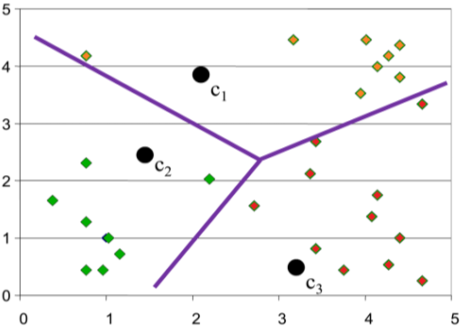
\includegraphics[width=150px]{img/HardClustering.png}
            \captionof{figure}{Grafik bei einem Hard Clustering}
            \label{fig:Grafik bei einem Hard Clustering}
        \end{Figure}

        \textit{Soft Clustering}
        \begin{itemize}
            \item Clusters können überlappen
            \item Stärke der Assoziation zwischen Clustern und Elementen (Wahrscheinlichkeit)
        \end{itemize}

    \section{Expectation Maximization (EM)}

    %ToDo: Übernehmen aus der Vorlesung 1

    \section{One-Class Classification}
    Die One-Class Classification wird auch als Ausreissererkennung, Neuheitserkennung oder Konzeptlernen bezeichnet. Dabei können unterschiedliche Algorithmen zum Zuge kommen:
    \begin{itemize}
        \item One-Class Support Vector Machine
        \item Clustering
        \item Decision Trees 
        \item Nerual Networks
        \item Bayesian Classifiers
    \end{itemize}
    \begin{Figure}
    \centering
    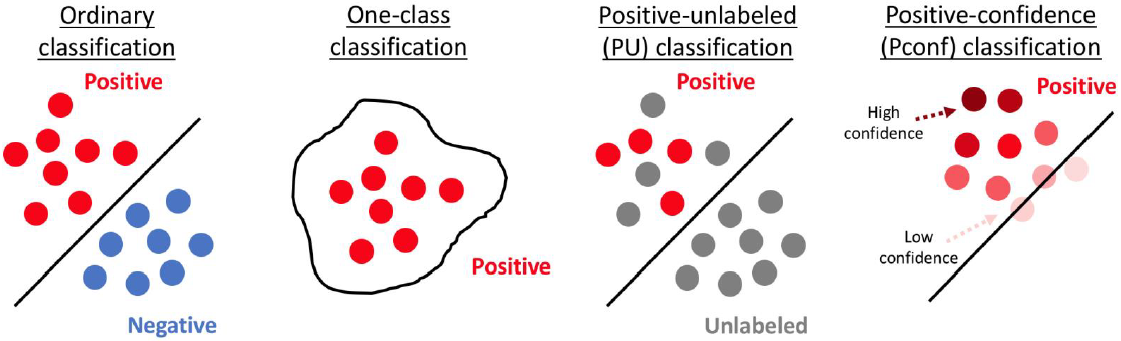
\includegraphics[width=150px]{img/ClassificationTasks.png}
        \captionof{figure}{Überblick über die verschiedenen Classification Tasks}
        \label{fig:Überblick über die verschiedenen Classification Tasks}
    \end{Figure}

    \section{Principal Component Analysis}
    $\Rightarrow$ Mit PCA verfolgen wir das Ziel eine reduzierte Form der Daten zu finden, welche die Daten möglichst gut erklären\\
    \begin{itemize}
        \item Es sind \textit{n} Sampels gegeben (werden auch \textit{oberservations} genannt)
        \item Für jedes sample haben wir \textit{m} Messungen (werden auch \textit{Dimensionen, Werte oder Variable} genannt)
        \item Dabei ist jede Messung eine reale Nummer
    \end{itemize}

    \subsection{PCA Plots}

		\subsubsection{Score Value}
        Der Score-Wert für eine Beobachtung, ist der Abstand vom Ursprung entlang der Richtung (loading vector) der ersten Komponenten bis zu dem Punkt, an dem diese Beobachtung auf den Richtungsvektor projiziert. Für jede Beobachtung (Zeile) im Datensatz gibt es einen Score-Wert, so dass es \textit{n} Score-Werte für die erste Komponenten, weitere \textit{n} Score-Werte für die zweite etc. gibt
        \begin{Figure}
        \centering
        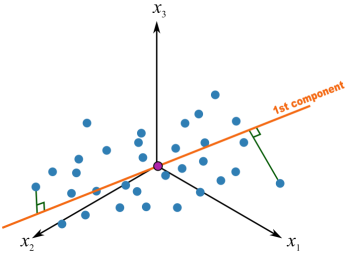
\includegraphics[width=150px]{img/ScoreValue.png}
            \captionof{figure}{Beispiel eines ScoreValues}
            \label{fig:Beispiel eines ScoreValues}
        \end{Figure}

		\subsubsection{Score Plot}
        In eime Score-Plot stellt man zwei Komponenten gegenüber um diese in einer zwei dimensionellen Grafik darzustellen. \\
        \textbf{Interpretation:}
        \begin{itemize}
            \item Ähnliche Samples sind nahe beieinander
            \item Durchschnittliche Samples werden nahe beim Ursprung liegen
            \item Outliers werden weit ausserhalb sein
        \end{itemize}	

		\subsubsection{Loading}
        \begin{itemize}
            \item Loading misst die Korrelation zwischen einer Komponenten und einer Variable
            \item Die Loading-Range ist von -1 bis 1
            \item Nahe bei -1 oder 1 $\Rightarrow$ Variable hat einen sehr starken Einfluss auf den Komponenten (+ oder - hat hier keine grosse Bedeutung)
            \item Nahe bei 0 $\Rightarrow$ Variable hat einen schwachen Einfluss auf die Komponenten
            \item Quadratische Belastungen geben den Anteil der Varianz der Variablen an, der durch die Komponenten erklärt wird
        \end{itemize}
        \begin{Figure}
        \centering
        \includegraphics[width=150px]{img/ScorePlotAndLoadingPlot.png}
            \captionof{figure}{Kombination eines Scores Plot mit einem Loading Plot}
            \label{fig:Kombination eines Scores Plot mit einem Loading Plot}
        \end{Figure}

	\subsection{Preprocessing for PCA}
    \begin{itemize}
        \item \textbf{Entferne Outliers:} bspw. wenn ein  Sensor nicht funktioniert und offenslichtlich falsche Resultate liefert
        \item \textbf{Skalierung:} Stelle sicher, dass alle Achsen in etwa die gleichen Werte haben
        \item \textbf{Centering:} Daten an den Ursprung des Koordinatensystems verschieben, indem der Mittelwert der Daten subtrahiert wird 
    \end{itemize}

		\subsubsection{Skalierung}
        \textbf{Problem:} Wenn Variablen sehr unterschiedliche Werte haben (z.B. Gewichte zwischen 70-100kg vs. Höhe zwischen 1.6-2.0m), hängt ihr Einfluss auf die PCA von diesen Werten ab\\
        \textbf{Ziel:} Alle Variablen (auf der X-Achse) haben in etwa die gleiche Grösse\\
        \textbf{Lösung:} Die am häufigsten verwendete Methode ist die Unit Variance Scaling , bei der jede Spalte durch ihre Standardabweichung geteilt wird. Dann wird jede Spalte eine Varianz von 1 haben.
        \begin{Figure}
        \centering
        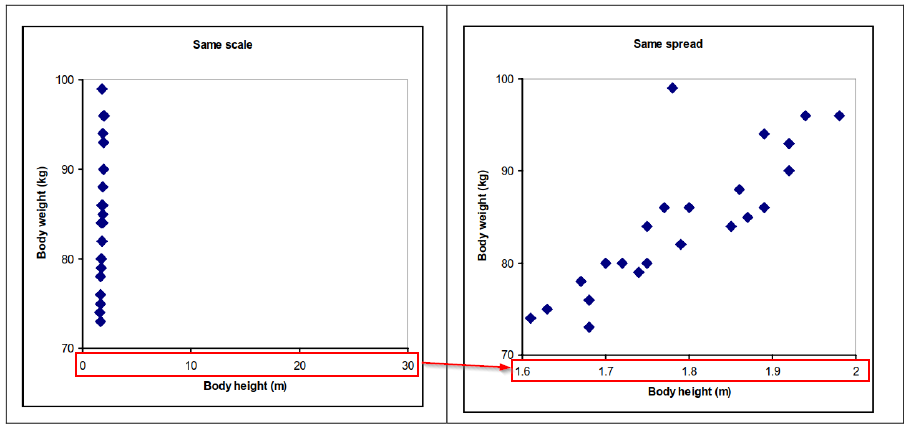
\includegraphics[width=150px]{img/Scaling.png}
            \captionof{figure}{Unterschied nach der Skalierung}
            \label{fig:Unterschied nach der Skalierung}
        \end{Figure}

		\subsubsection{Centering}
        \textbf{Ziel:} Das Koordinatensystem vom Ursprung zu einem neuen Referenzpunkt verschieben, so dass die Beobachtungen um den neuen Punkt herum verstreut sind\\
        \textbf{Lösung:} den Mittelwert aller Datenpunkte von jedem Datenpunkt subtrahieren\\
        \textbf{Alternativ:} Mediane Zentrierung, da diese robuster gegenüber Ausreissern ist
        \begin{Figure}
        \centering
        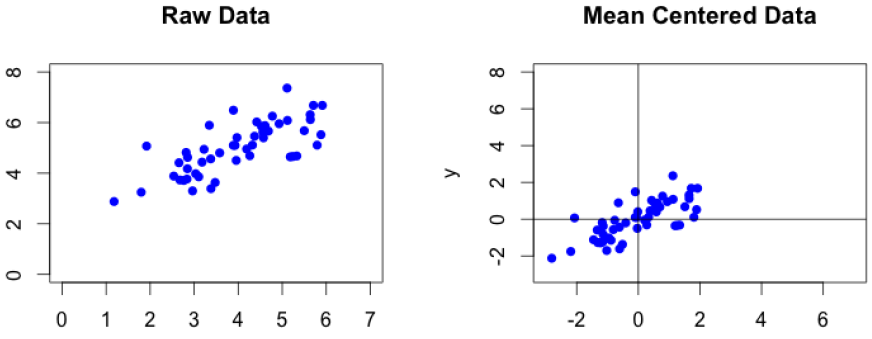
\includegraphics[width=150px]{img/Centering.png}
            \captionof{figure}{Unterschied der beiden Möglichkeiten nach der Zentrierung}
            \label{fig:Unterschied der beiden Möglichkeiten nach der Zentrierung}
        \end{Figure}

	\subsection{Auswahl der Principal Components}
    \begin{itemize}
        \item \textbf{Daumenregel:} 2-5 Principal Components sind üblicherweise genügend
        \item \textbf{Kaiser's Rule:} Wähle alle Components wo der Eigenvalue grösser als 1 ist
        \item \textbf{Prozentsatz der Cumuluative Varianz} siehe Unterkapitel
        \item \textbf{scree Plot:} Nehmen Sie die Komponenten, die sich vor dem Abflachen der Neigung befinden $\Rightarrow$ Ellbow
    \end{itemize}

		\subsubsection{Cumuluative Varianz}
        Die kumulative Varianz (k) ist die Varianz, welche durch den ersten k PC erklärt wird
        \textit{Berechnung}:
        \begin{equation}
            \sum^{k}_{i=1} \frac{\lambda_i}{\sum^{m}_{j=1} \lambda_j}
        \end{equation}

    \section{Keyphrase Extraction (RAKE)}
    Die Hauptaufgabe ist \textit{Finde möglichst gute Schlüsselwörter für ein Text-Dokument}, diese Aufgabe kann man in unterschiedlichen Varianten lösen:
    \begin{itemize}
        \item Keyphrase Extraction: nur einzelne Wörter aus dem Text
        \item Keyphrase Extractino: ein oder mehrere angrenzende Wörter aus dem Text
        \item Main Topic Identification: Erlaubt sogar Begriffe, welche nicht im Text stehen
    \end{itemize}
    \begin{Figure}
    \centering
    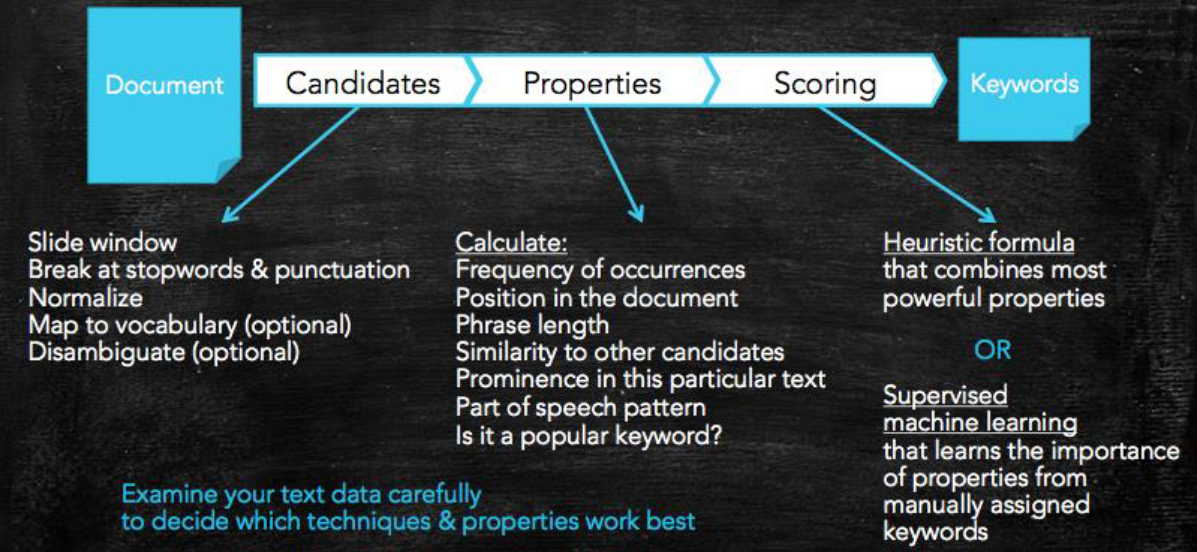
\includegraphics[width=150px]{img/MainPrincipeKeyphraseExtraction.png}
        \captionof{figure}{Hauptprinzip der Keyphrase Extraction}
        \label{fig:Hauptprinzip der Keyphrase Extraction}
    \end{Figure}

		\subsubsection{Rapid Automatic Keyword Extraction (RAKE)}
        RAKE ist ein Algorithmus um Schlüsselwörter in einem Text zu identifzieren. 
        \begin{itemize}
            \item Kandidat, wenn Wort zwischen zwei Stoppwörter oder Satzzeichen stehen
            \item Parameters: 1. Stopword list; 2. Minimale Wortlänge (bspw. 4 char); 3. maximale Phrase-Länge (bspw. 3 Wörter)
            \item Output $\Rightarrow$ eine Liste mit Phrasen, sortiert nach dem Phrase-Score
        \end{itemize}

        \textbf{Scoring}:\\
        \t \textit{Durchschnittswerte:}
        \begin{itemize}
            \item degree(phrase) $\rightarrow$ Anzahl Wörter im Satz 
            \item frequency(word) $\rightarrow$ Anzahl der Wort-Häufigkeit im gesamten Text
            \item degree(word) $\rightarrow$ Summe von degree(phrase) über alle Sätze wo das entsprechende Wort beinhalten
            \item score(word)
        \end{itemize}

        \t \textit{RAKE Score:}
        \begin{itemize}
            \item score(phrase) $\rightarrow$ Summe von allen score(word) für jedes Wort im Satz
        \end{itemize}
    
    \section{TF-IDF}
    Die Problematik ist, dass Wörter die sehr häufig vorkommen, nicht zwingend sehr relevant sind.
    \begin{Figure}
    \centering
    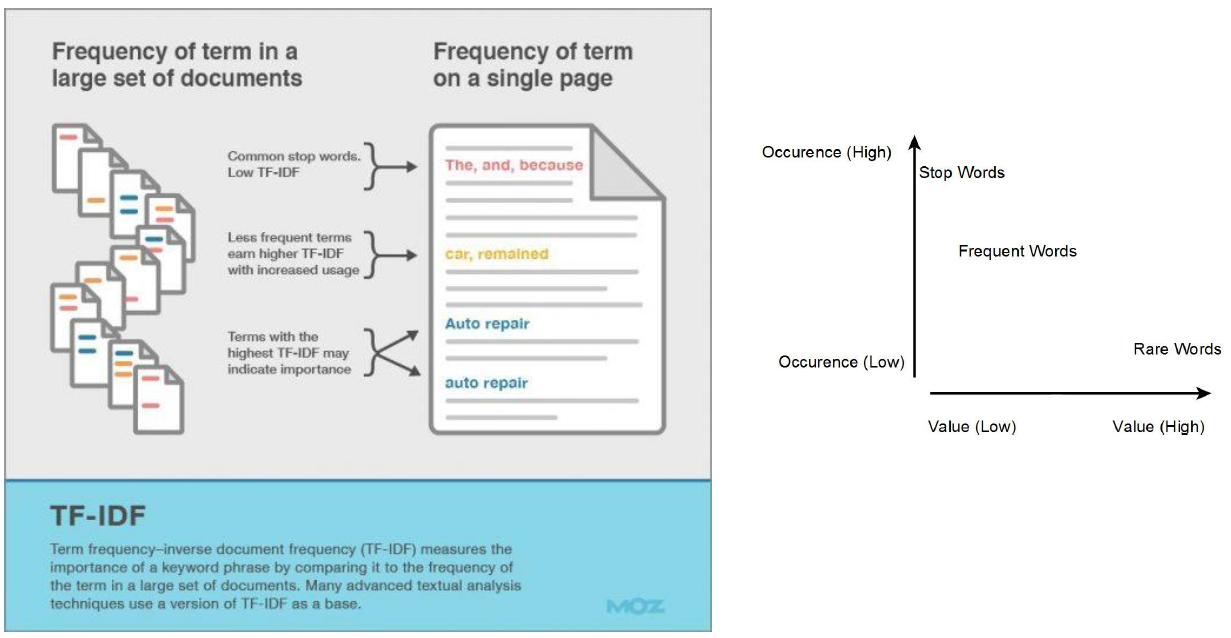
\includegraphics[width=150px]{img/WordImportance.png}
        \captionof{figure}{Häufigkeit der Wörter in Bezug auf ihre Relevanz}
        \label{fig:Häufigkeit der Wörter in Bezug auf ihre Relevanz}
    \end{Figure}
    
    Dabei kann TF-IDF (\textbf{Term Frequency - Inverse Document Frequency}) abhilf schaffen.
    \begin{equation}
        w_{x , y} = tf_{x , y} * log(\frac{N}{df_x})
    \end{equation}

    Dies beschreibt wie häufig der Begriff \textit{x} im Dokument \textit{y} vorkommt.\\
    $tf_{x , y}$ = Häufigkeit von \textit{x} in \textit{y}\\
    $df_x$ = Anzahl von Dokumenten die \textit{x} enthalten\\
    $N$ = Total Anzahl Dokumente\\
    $\Rightarrow$ Daraus resuliert dann eine TF-IDF-Liste, welche bereits den Korrekturfaktor miteinberechnet.
    \begin{Figure}
    \centering
    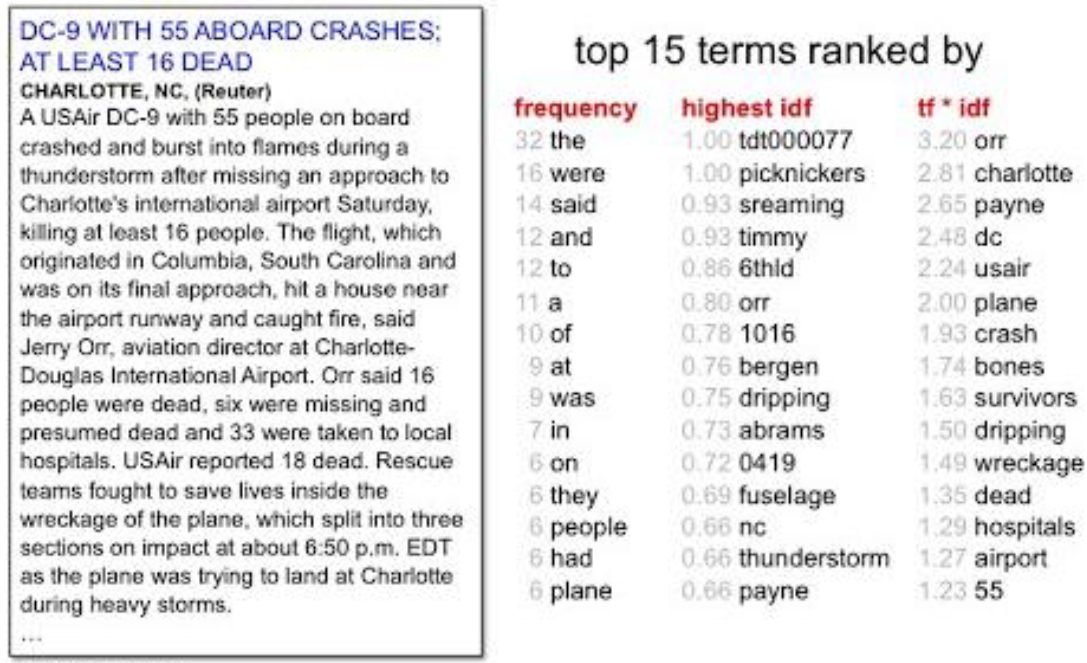
\includegraphics[width=150px]{img/tfidfexample.png}
        \captionof{figure}{Beispiel einer TF-IDF-Liste}
        \label{fig:Beispiel einer TF-IDF-Liste}
    \end{Figure}

    \section{Topic Modeling (LDA)}
    Das Hauptziel ist, Dokumente im Kontext eines grossen Korpus (Textbestandes) zu erforschen.\\
    'Verstehe' ein einziges Dokument $\rightarrow$ Finde 'ähnliche' Dokumente $\rightarrow$ Liefere besseres Suchresultat

	    \subsection{Was ist ein Topic?}
        \begin{itemize}
            \item Eine Gruppe von Wörter, bei denen es eine sehr hohe Wahrscheinlichkeit gibt, dass sie im gleichen Kontext erscheinen
            \item Syntax wird nicht betrachtet
            \item Kann nur auf Nomen eingeschränkt werden, ist aber nicht notwendig
            \item Eine verborgene Struktur, mit deren Hilfe bestimmt werden kann, welche Wörter wahrscheinlich in einem Text vorkommen
        \end{itemize}

        \subsection{Anwendungen}
        \begin{itemize}
            \item Bessere Suchresultate $\rightarrow$ Suche nach 'genome' und liefere Dokumente die 'DNA', 'genes' oder 'RNA' zurückliefert (mehr wie nur Synonyme)
            \item Erhalte einen Überblick über grosse Dokumentenmengen
            \item Ein einzelnes Dokument mit einer riesigen Sammlung von Dokumenten in Zusammenhang bringen 
        \end{itemize}

        \begin{Figure}
        \centering
        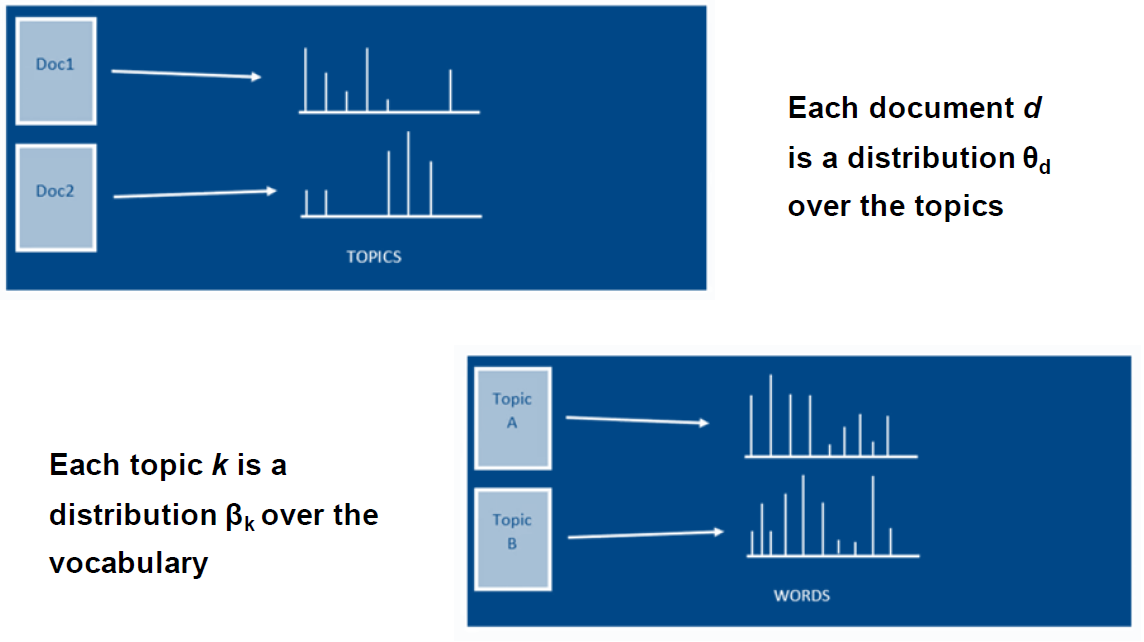
\includegraphics[width=150px]{img/ProbabilisticTopicModel.png}
            \captionof{figure}{Probabilistic Topic Model}
            \label{fig:Probabilistic Topic Model}
        \end{Figure}

	    \subsection{Probabilistic Generative Process}
        Grundidee:
        \begin{itemize}
            \item \textbf{Gegeben} eines festen Vokabulars und einer Reihe von \textit{K}-Themen. Jedes Thema ist eine Wahrscheinlichkeitsverteilung über das Vokabular
            \item Um ein Dokument zu \textbf{erstellen}, wählt man zunächst die Textlänge, die Anzahl der Wörter und eine Verteilung auf die Themen (z.B. Thema1 60-Prozent, Thema2 40-Prozent)
            \item Für jedes Wort im Dokument \textbf{wählt man zufällig} das Thema entsprechend der Themenverteilung (z.B. Thema1), dann \textbf{wählt man zufällig} ein Wort aus dem Vokabular entsprechend der Themenverteilung im Vokabular (z.B. Affe)
        \end{itemize}
        $\Rightarrow$ Es kann verwendet werden um (theoretisch) Texte zu erstellen anhand der Topic-Verteilung, dies war für die LDA fundamental wurde in der Realität jedoch nie verwendet.

        \begin{Figure}
        \centering
        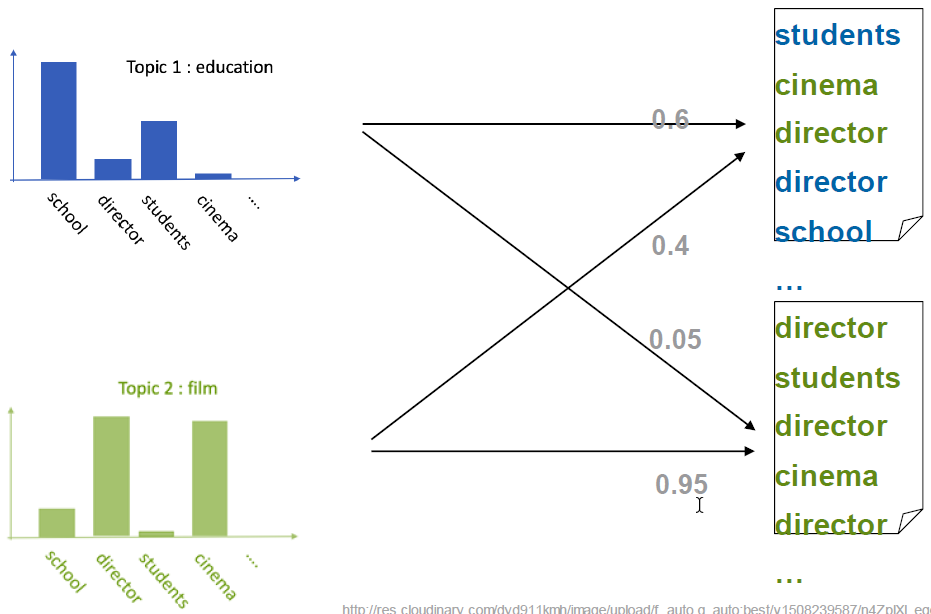
\includegraphics[width=150px]{img/GenerativeProcessExample.png}
            \captionof{figure}{Ein Beispiel für ein Generative Process}
            \label{fig:Ein Beispiel für ein Generative Process}
        \end{Figure}

	    \subsection{LDA}
        LDA = Latent Dirichlet Allocation, mit dem Hauptziel \textit{wir beobachten nur die Dokumente und ihre Worte, und unser Ziel ist es, auf die zugrunde liegende Themenstruktur zu schließen}
        \begin{itemize}
            \item \textbf{Latent} $\rightarrow$ Die zugrunde liegende Struktur ist unbekannt
            \item \textbf{Dirichlet} $\rightarrow$ sind die angenommenen Wahrscheinlichkeitsverteilungen des Themas und der Wörte
            \item \textbf{Allocation}$\rightarrow$ weil es die wahrscheinlichste Lösung auf der Grundlage der Daten zuweist
        \end{itemize}

		    \subsubsection{Grundidee des LDA-Algorithmus}
            Dabei handelt es sich um ein Expectation-Maximization-Algorithmus.\\

            Gegeben sei ein Set \textit{D} von Dokumenten.\\
            \textbf{Ablauf:}
            \begin{enumerate}
                \item Fix the number of topics \textit{K}
                \item Randomly initialize estimates of the hidden parameters $\theta_d$ and $\beta_k$
                \item Repeat $\rightarrow$ 1. Use estimated probabilities to assign topics to each document $\rightarrow$ 2. Use estimated probabilities and topic assignments to assign topics to each single word $\rightarrow$ 3. Update estimates based on the topic-to-word assignments
                \item $\Rightarrow$ Bis Prozess konvergiert
            \end{enumerate}

                    \subsubsection{anwenden von LDA}
            \begin{enumerate}
                \item Entferne irrelevanten Text
                \item Sammle alle Wörter und sortiere dies nach der Frequenz
                \item Reduziere die Wortliste (bspw. wenn ein Wort mehr als in 10% aller Texte vorkommt, Wortlänge etc.)
                \item Lemmatization or stemming
                \item Behalte die Top-Wörter (bspw. 50000 - 100000)
                \item Verwende bag-of-words oder TF-IDF als input für LDA
                \item Variiere mit den Hyperparameters von LDA (bspw. Anzahl TOpics oder Dirichlet parameter)
                \item manuelle Qualitätsanalyse der Themen und Themenzuweisung
            \end{enumerate}

\chapter{Supervised Learning}

    \section{Linear Regression}
    Die Linear Regression wird verwendet um eine Beziehung zwischen zwei fortlaufenden Variablen aufzuzeigen.\\
    Beispiele:
    \begin{itemize}
        \item Grösse und Gewicht $\rightarrow$ Wenn man grösser ist, erwartet man, dass man auch schwerer ist
        \item Alkoholkonsum und Alkoholgehalt im Blut 
        \item Wie schnell man fährt und Benzinverbrauch
    \end{itemize}
    $\Rightarrow$ Wenn es keine Beziehung zwischen den Variablen gibt oder es sich um eine deterministische Beziehung handelt, ist dies nicht geeignete für lineare Regression

    \begin{Figure}
    \centering
    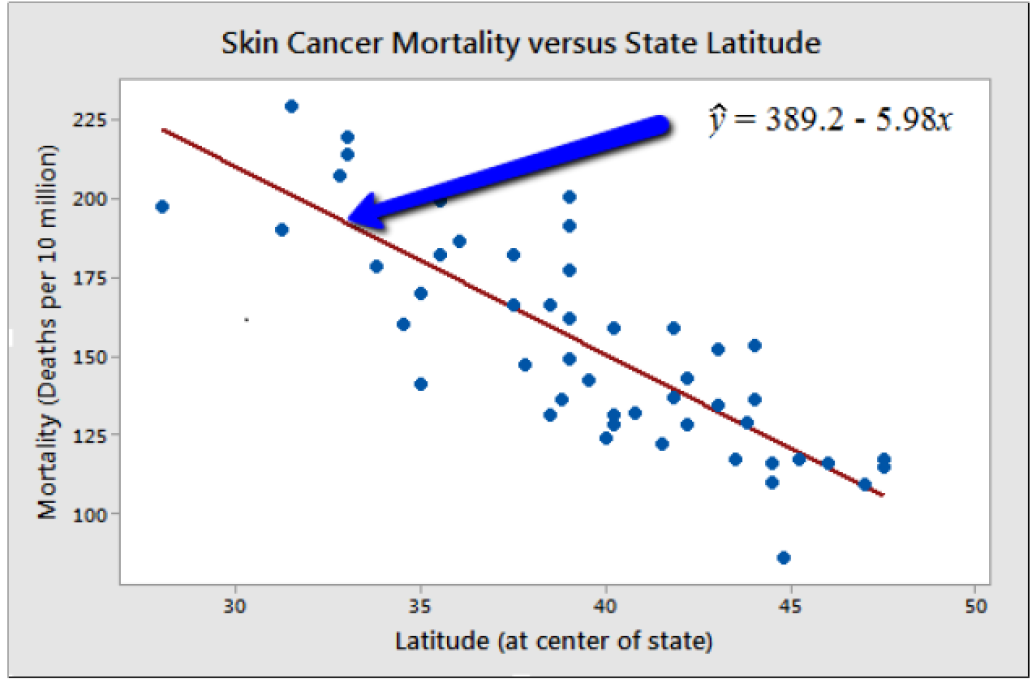
\includegraphics[width=150px]{img/LinearRegressionExample.png}
        \captionof{figure}{Ein Beispiel für die lineare Regression}
        \label{fig:Ein Beispiel für die lineare Regression}
    \end{Figure}
        \subsection{Bivariate vs. Multivariate Modelle}

    \begin{Figure}
    \centering
    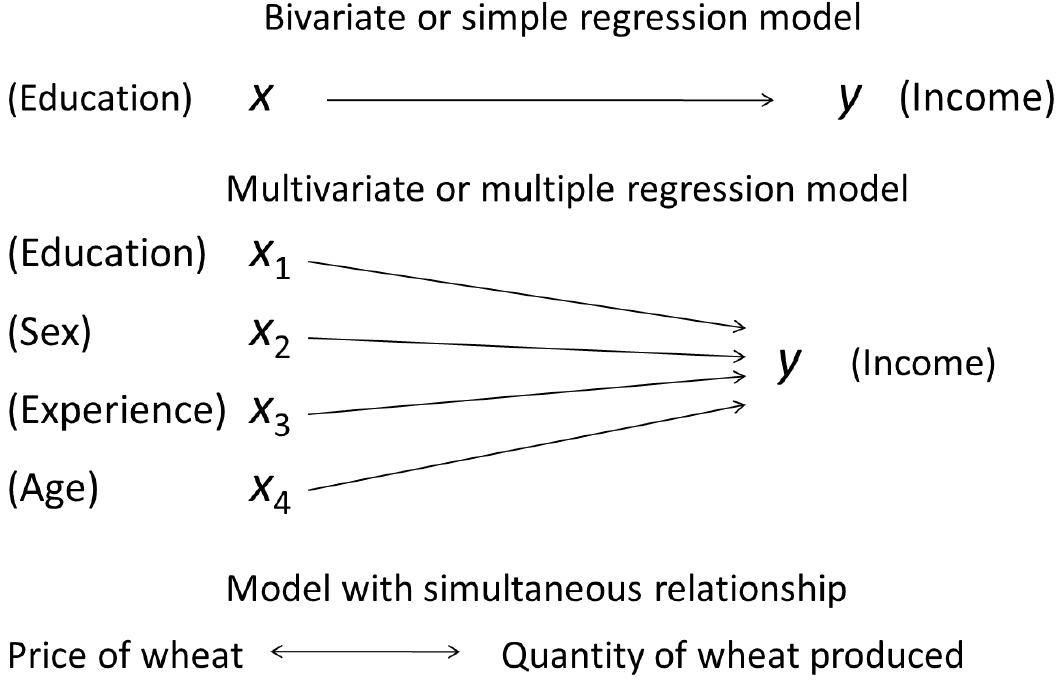
\includegraphics[width=150px]{img/BiMultivariate.png}
        \captionof{figure}{Ein Beispiel für den Unterschied von Bivariate und Multivariate Modelle}
        \label{fig:Ein Beispiel für den Unterschied von Bivariate und Multivariate Modelle}
    \end{Figure}
    
        \subsection{Simple Linear Regression (SLR)}
        Das Hauptziel von SLR ist die Parameter \textit{a} und \textit{b} der linearen Funktion zu finden, sodass sich der \textit{Mean Squarred Error (MSE)} minimiert
        \begin{itemize}
            \item \textbf{Variable X-Achse}: Wird als \textit{explanatory} oder \textit{predictor} oder \textit{unabhängige Variable} bezeichnet
            \item \textbf{Variable Y-Achse}: Wird als \textit{response} oder \textit{criterion} oder \textit{abhängige Variable} bezeichnet
        \end{itemize}
        \textbf{Model:}
        \begin{equation}
            y^{i} = ax^{i} + b \epsilon^{i}
        \end{equation}
        \begin{itemize}
            \item \textbf{i} sind die Beispiele / Samples
            \item \textbf{a} ist die Steigung der linearen Regression
            \item \textbf{b} wird als \textit{y-interceptor} betitelt
            \item \textbf{$\epsilon^{i}$} ist ein zufälliger Fehler (anhand der Normalverteilung)
        \end{itemize}

            \subsubsection{Mean Squarred Error}
            Für gegebenes a und b, sei $\^{y}^{(i)} = ax^{(i)} + b$ der vorhergesagte Wert
            \begin{equation}
                MSE = \frac{1}{m} \sum^m_{i=1} (\^{y}^{(i)} - y^{(i)})^2
            \end{equation}

            \begin{Figure}
            \centering
            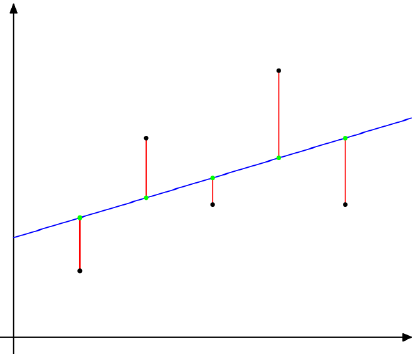
\includegraphics[width=150px]{img/GoalSLR.png}
                \captionof{figure}{Ein Beispiel für den Unterschied von Bivariate und Multivariate Modelle}
                \label{fig:Ein Beispiel für den Unterschied von Bivariate und Multivariate Modelle}
            \end{Figure}
            
            \subsubsection{Korrelation}
            Der \textit{Pearson Correlation Coefficient} misst die Stärke der Beziehung zwischen den zwei quantitativen Variablen.
            \begin{equation}
                r = \frac{1}{m-1} \sum^m_{i=1} (\frac{x^{(i)} - \bar{x}}{s_x}) (\frac{y^{(i)} - \bar{y}}{s_y})
            \end{equation}
            Wobei
            \begin{itemize}
                \item $\bar{x}$ und $\bar{y}$ die Stichprobenmittelwerte der x- und y-Variablen sind
                \item $s_x$ und $s_y$ die Standardabweichung von x und y sind
            \end{itemize}
		
            \subsubsection{Berechnung von SLR}
            Die Variablen a und b minimieren den Mean Square Error
            \begin{equation}
                a = \frac{\sum^m_{i=1}x^{(i)}y^{(i)} - \bar{y}m\bar{x}}{\sum^m_{i=1} x^{(i)^{2}} - \bar{x} \sum^m_{i=1} x^{(i)}} = r \frac{s_y}{s_x} \t b=\bar{y} - a\bar{x}
            \end{equation}
            \textbf{Idee:}
            \begin{itemize}
                \item Berechnen Sie partielle Ableitungen von MSE in Richtung a und b
                \item Setzen Sie diese auf Null, verwenden Sie Kalkül, um das Gleichungssystem zu lösen
                \item Zweite Gleichheit für a: verwendet die Standardabweichung s x und s y und den Pearson-Korrelationskoeffizienten r zwischen x und y siehe Definition auf dem nächsten Bild )
            \end{itemize}

            \subsubsection{Grundlegende Annahmen in SLR}
            \begin{enumerate}
                \item Ein lineares Modell passt zu dem Problem
                \item Die Beobachtungen sind voneinander unabhängig
                \item Alle notwendigen unabhängigen Variablen sind im Modell enthalten
                \item Die Fehlerbegriffe $\epsilon_1$ are normal verbreitet
                \item Fehler zwischen verschiedenen Beobachtungen haben eine konstante Varianz Homokedastizität
            \end{enumerate}
                    
            \subsubsection{Residual}
            Das Residuendiagramm ist ein Streudiagramm von vorhergesagten Werten vs. Residuen.\\
            Das Residual für die Beobachtung \textit{i} ist gegeben durch $e^{(1)} = y^{(i)} - \^{y}^{(i)}$
            
            \subsubsection{Multivariate Linear Regression}
            Zurvor haben wir uns mit der Formel $y = ax + b$ bekannt gemacht.\\
            
            Allgemeiner ausgedruckt wird die Formel wie folgt: $h_{\theta}(x) = \theta_0 + \theta_1 x_1 + \theta_2 x_2 + ... + \theta_n x_n$
            \begin{itemize}
                \item n steht für die Anzahl von Variablen (=measurements)
                \item m steht für die Anzahl von Samples (hier nicht aufgeführt)
                \item $h_{\theta}$ ist die Hypothese mit den Parametern $\theta_0$ etc.
            \end{itemize}
            
                    \subsubsection{Kostenfunktion}
            \textbf{Ziel:} Wir wollen $\theta$ so wählen, dass wir J($\theta$) minimieren $\rightarrow$ möglichst wenig Kosten generieren.\\
            \textbf{Idee:}
            \begin{enumerate}
                \item Initialisiere $\theta$ (bspw. zufällig oder durch raten)
                \item Wiederholend $\theta$ anpassen um J($\theta$) zu verkleinern
                \item Durchführen bis Konvergenz erreicht wurde
            \end{enumerate}
            \textbf{Formel:}
            \begin{equation}
                J(\theta) = \frac{1}{2} \sum^m_{i=1} (h_{\theta}(x^{(i)}) - y^{(i)})^2 
            \end{equation}

    
    \section{Gradient Descent}
    \textbf{Idee:} Verwendung von Gradienten von $\theta$ um seinen Wert bei jedem Schritt zu adaptieren
    \begin{equation}
        \theta_j := \theta_j - \alpha \frac{\partial}{\partial \theta_j} J(\theta)
    \end{equation}
    Wobei hier $\alpha$ die Learning-rate ist. Die Learning rate ist durchaus wichtig im gesamtem Prozess. Ist sie zu klein, so konvergiert es nur sehr langsam. Ist sie zu gross, so überschiesst sie allenfalls das Ziel und findet entsprechend die eigentliche Lösung nicht.

        \subsection{High-Order Linear Regression}
    Ein weiteres Problem haben wir, wenn wir nicht linearen Daten uns annähern wollen.\\
    \textbf{Vorgehen:} Man nimmt den eindimensionalen input-wert z und projiziert diesen auf eine höhere Dimension, so dass die lineare Funktion auch kompliziertere Beziehungen zwischen x und y anpassen kann.
    \textbf{Beispiel:}
    \begin{itemize}
        \item Der Input ist z (ein-dimensional)
        \item Definiere eine Transformation $x_k := f_k(z) = z^{2*k}$ für k = 1, 2, 3, 4
        \item lineares Modell: $h(x) = \theta_0 + \theta_1 x_1 + \theta_2 x_2 + \theta_3 x_3 + \theta_4 x_4 = \theta_0 + \theta_1 z^2 + \theta_2 z^4 + \theta_3 z^6 + \theta_4 z^8$
        \item $\Rightarrow$ Das Modell ist polynomial in z, aber linear in x
    \end{itemize}

    \section{Logistic Regression}
    Die Logistic Regression löst einen Classification Task.\\
    Gegegeben:
    \begin{itemize}
        \item Given are m training examples $(x^{(i)}, y^{(i)})$
        \item Jedes $x^{(i)}$ ist ein n-dimensionaler Feature-vector
        \item $y^{(i)} \in \{0,1\}$
    \end{itemize}

    \section{Support Vector Machines}
    \textbf{Ziel:} Eine Hyperebene finden, die die beiden Klassen von Eingabepunkten mit maximalem Spielraum trennt
    \begin{Figure}
    \centering
    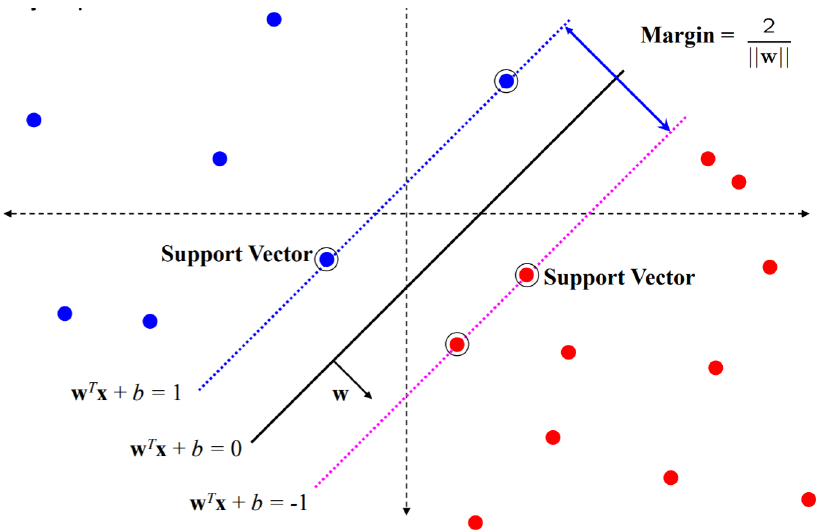
\includegraphics[width=150px]{img/SVMSetting.png}
        \captionof{figure}{Support Vector Machine}
        \label{fig:Support Vector Machine}
    \end{Figure}

        \subsection{Regulierung}
    \begin{itemize}
        \item Was ist der beste Abstand? $\rightarrow$ Meisten gibt es einen Kompromiss zwischen dem Abstand und der Anzahl Fehler auf den Trainingsdaten
        \item Soft-Margin $\rightarrow$ evtl genauer anschauen %Todo
    \end{itemize}

%ToDo Kernel Trick ergänzen

    \section{Corpus Construction}
%ToDo Corpus Construction weiter ausführen
    \textbf{Inter-Annotator Agreement}\\
    Misst inwiefern sich zwei Annotatoren einigen sind bezg. dem Data-Label:
    \begin{equation}
        K = \frac{n_{shared} - n_{random}}{1-n_{random}}
    \end{equation}
    \begin{itemize}
        \item grösser als 0.7 ist ein guter Wert, kleiner als 0.4 ist ein schlechter Wert
    \end{itemize}   

    \section{Word Embeddings}
    

    \section{Algorithm Selection}
	    \subsection{Word Vectors}
        \begin{itemize}
            \item Jeder Wort wird durch einen Vektor repräsentiert
            \item die Repräsentation wird durch den gegebenen Text und das Wort selbst, berechnet
        \end{itemize}
                \subsubsection{Bag of Words}
        \textbf{Bag of Words} ist eine traditionelle Form wie man die Wörter repärsentieren kann.
        \begin{itemize}
            \item Jedes Wort hat eine ID, die Position im Wörterbuch von allen Wörter
            \item Vektorlänge ist gleich der Anzahl Wörter im Wörterbuch
            \item Trägt eine 1 an, wenn es sich um das Wort handelt, sonst 0
        \end{itemize}

        \begin{Figure}
        \centering
        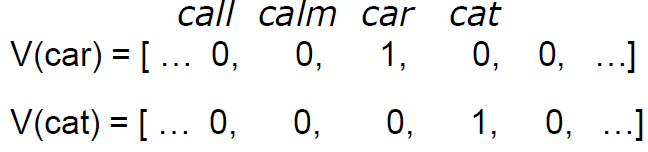
\includegraphics[width=150px]{img/BOW.png}
            \captionof{figure}{Beispiel einer Bag of Words Repräsentation}
            \label{fig:Beispiel einer Bag of Words Repräsentation}
        \end{Figure}
        \begin{Figure}
        \centering
        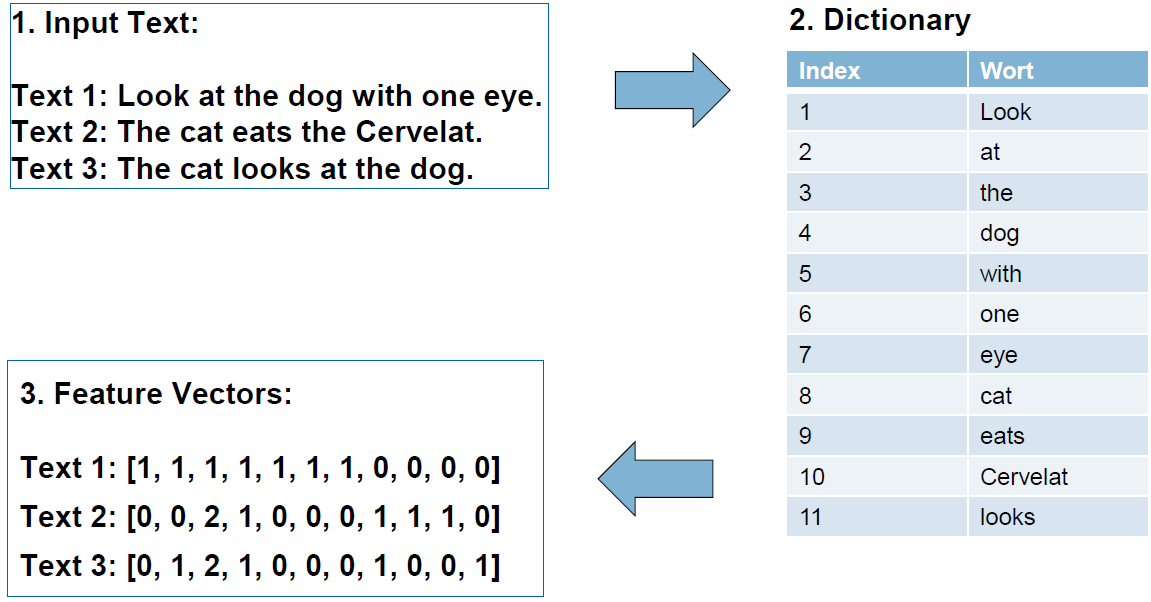
\includegraphics[width=150px]{img/BOW2.png}
            \captionof{figure}{Ablauf einer Bag of Words Repräsentation}
            \label{fig:Ablauf einer Bag of Words Repräsentation}
        \end{Figure}

            \subsubsection{Neural Word Embeddings}
            Einfache String als Input funktioniert wirklich gut, daher muss man sich für Text-Analyse etwas mehr gedanken machen. \\
            \begin{itemize}
                \item Multidimensionale Repräsentationen von Wörter
                \item 50-300 Dimensionen sind häufig normal
                \item werden auf Basis eines neuronalen Netzwerkes berechnet
                \item Haben eine dichte Repräsentation (wenig Nullen)
                \item Encoden eine semantische Ähnlichkeit (bspw. Synonyme)
                \item Encoden Analogien (bspw. Distanz zwischen King und Queen ist identisch wie die Distanz zwischen Frau und Mann)
            \end{itemize}

	    \subsection{Welcher Algorithmus soll nun gewählt werden}
        \textbf{Kriterien:}
        \begin{itemize}
            \item Genauigkeit
            \item Trainingszeit
            \item Parameter
        \end{itemize}
        $\Rightarrow$ Es gibt nicht den einen perfekten Algorithmus, sondern es muss je nach Anwendungsfall unterschieden werden $\rightarrow$ No Free Lunch Theorem

        \subsection{Daten}
        Typischerweise splitet man sein Trainingsset in 70\% Train, 20\% Validation und 10\% Test

        \begin{Figure}
        \centering
        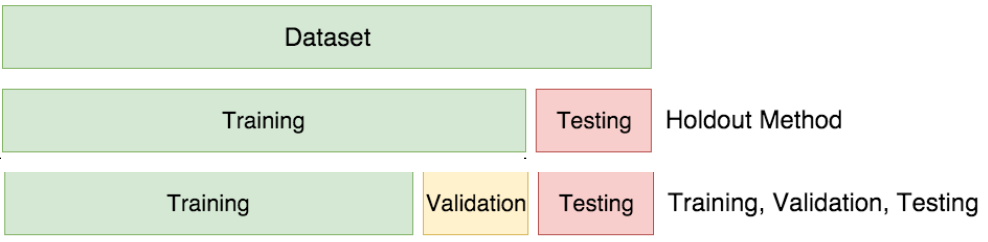
\includegraphics[width=150px]{img/TrainValTest.png}
            \captionof{figure}{Aufsplittung der Daten}
            \label{fig:Aufsplittung der Daten}
        \end{Figure}

	    \subsection{Cross-Validation}
        \begin{itemize}
            \item Die Trainingsdaten werden in disjunkte Fold eingeteilt
            \item Trainiere auf einigen Fold, evaluiere mit den anderen
            \item Durchschnittlicher Wert nach allen Experimenten
            \item Typische Varianten: \textit{Leave One Out Cross Validation} oder \textit{k-fold Cross Validation}
        \end{itemize}
        \begin{Figure}
        \centering
        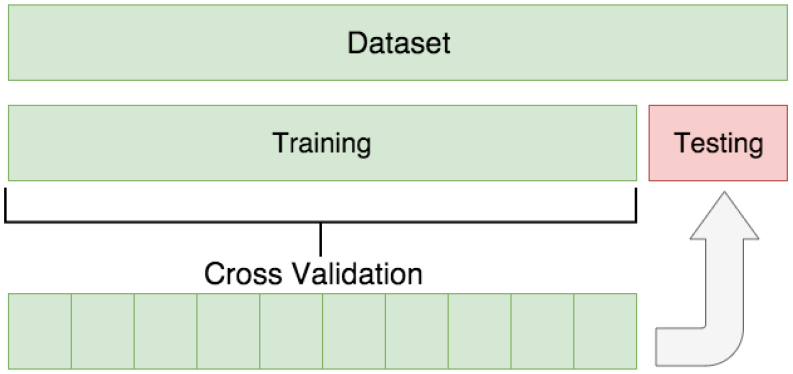
\includegraphics[width=150px]{img/Cross-Validation.png}
            \captionof{figure}{Schema Cross Validation}
            \label{fig:Schema Cross Validation}
        \end{Figure}

		    \subsubsection{Leave One Out Cross Validation}
            \begin{itemize}
                \item Jedes Trainingsbeispiel ist ein einzelner Fold
                \item Für jeden Fold F, wird das Modell auf allen (ausser F) trainiert und anschliessend auf F getestet
                \item Durchschnittswert gilt 
                \item $\rightarrow$ Berechnung ist sehr teuer, nur mit kleinen Datensets verwenden
            \end{itemize}

            \subsubsection{k-fold Cross Validation}
            \begin{itemize}
                \item Verwende ein zufälliges \textit{k} an Subsets der Trainingsdaten
                \item bspw. k=10
            \end{itemize}
            \begin{Figure}
            \centering
            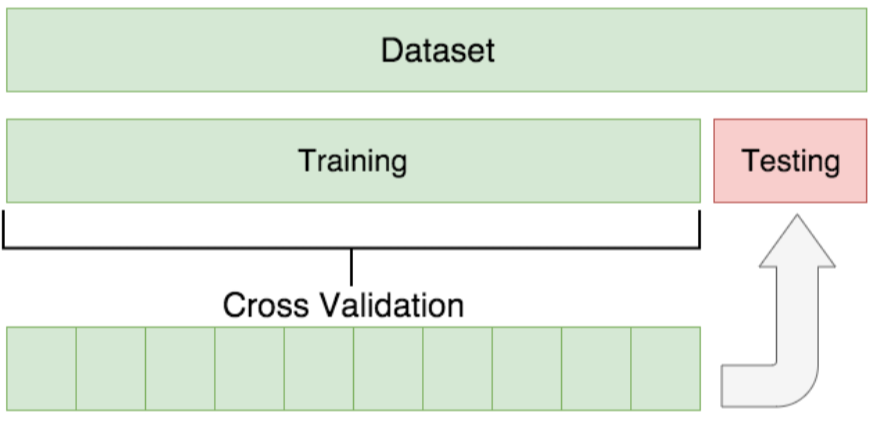
\includegraphics[width=150px]{img/Cross-kFoldCV.png}
                \captionof{figure}{Schema k-Fold Cross Validation}
                \label{fig:Schema k-Fold Cross Validation}
            \end{Figure}


    \section{Quality Measurements}
    \textbf{Genauigkeit}
    \begin{equation}
        Accuracy = \frac{correctDocuments}{allDocuments}
    \end{equation}

    \textbf{Confusion Matrix}
    \begin{Figure}
    \centering
    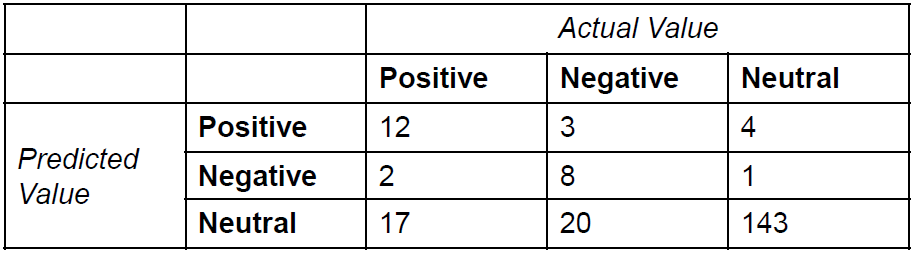
\includegraphics[width=150px]{img/ConfusionMatrix.png}
        \captionof{figure}{Abbildung einer Confusion Matrix}
        \label{fig:Abbildung einer Confusion Matrix}
    \end{Figure}

    \textbf{Präzision für positive Dokumente}: P_pos = true positives / (true positivies + false positivies)\\
    \textbf{Recall für positive Dokumente}: R_pos = true positives / all positive document

        \subsection{F-Score}
    A balanced combination of Precision and Recall\\
    \textbf{General F-Score:} $F_\beta = (1 + \beta^2) * \frac{precision * recall}{(\beta^2 * precision) + recall}$ \\
    \textbf{F1 Scores uses $\beta = 1$:} $F_1 = 2 * \frac{precision * recall}{precision + recall}$\\
    For sentiment analysis, the F1-Score of the resulting classes (positive and negative) is usually averaged: $F = \frac{F_{pos} + F_{neg}}{2}$


    \section{Learning Curve Analysis}
    Bewerten Sie Tendenzen des Trainings und Testkurven für genügend Beispiele.
    \textbf{Grundregeln:}
    \begin{itemize}
        \item Wenn beide Kurven "nahe beieinander" liegen und beide eine niedrige Punktzahl haben --> potentielle \textbf{underfitting} (High Bias)
        \item Wenn die Trainingskurve ein viel besseres Ergebnis als die Testkurve hat --> mögliche overfitting (hohe Varianz)
    \end{itemize}
    \begin{Figure}
        \centering
        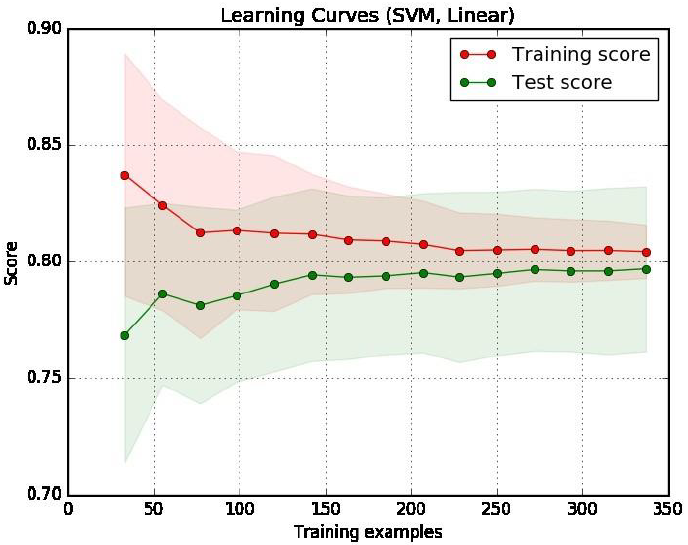
\includegraphics[width=150px]{img/LearningCurve.png}
            \captionof{figure}{Abbildung einer Learning Curve}
            \label{fig:Abbildung einer Learning Curve}
    \end{Figure}

\chapter{Neural Networks}
    \section{Neural Networks in a Nutshell}
    Die ersten Ansätze von Neuronalen Netzwerk gehen auf die 40er Jahre zurück. Wobei man mehrere Inputs hatte, diese Gewichtet und verknüpft hat und anschliessend einen Output erhalten hat.\\
    anschliessend kam \textit{The Perceptron} welcher die Grundidee aufnahm adaptive (trainierbare) Gewichtungen miteinfliessen zu lassen.
    \begin{Figure}
    \centering
    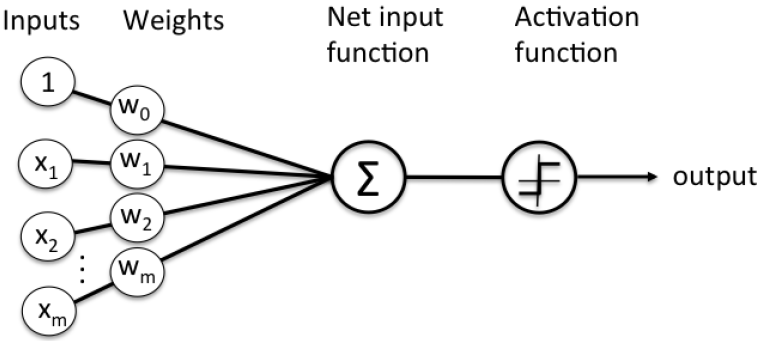
\includegraphics[width=150px]{img/ThePerceptron.png}
        \captionof{figure}{Abbildung vom Perceptron}
        \label{fig:Abbildung vom Perceptron}
    \end{Figure}
    Als Weiterentwicklung kam der Multilayer Perceptron in den 60er Jahre, war jedoch noch sehr ineffizient zum Trainieren
    \begin{Figure}
    \centering
    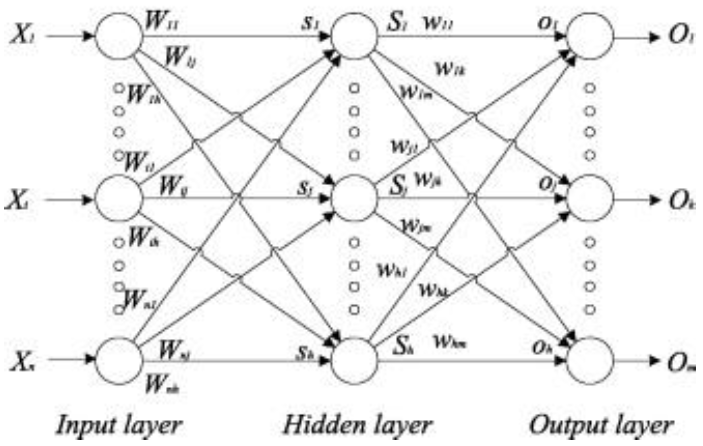
\includegraphics[width=150px]{img/MLP.png}
        \captionof{figure}{Abbildung vom Multi-Layer Perceptron}
        \label{fig:Abbildung vom Multi-Layer Perceptron}
    \end{Figure}

    \section{Perecptrons}
    \textbf{Neuron aus biologischer Sicht}
    \begin{itemize}
	    \item Ein Neuron ist mit anderen Neuronen über ca. 10000 Synapsen verbunden
	    \item Sobald der Input einen kritischen Wert überschreitet, entlädt das Neuron eine Spitze eines elektrischen Impulses, der vom Körper durch das Axon hinunter zum nächsten Neuron (zu den nächsten Neuronen) wandert.
	    \item Die Axonenden berühren fast die Dendriten oder den Zellkörper des nächsten Neurons.
    \end{itemize}

    \textbf{Die technische Sicht - weshalb künstliche Intelligenz}
    \begin{itemize}
        \item \textbf{Technischer Aspekt} $\rightarrow$ Einige Probleme wie die Zeichenerkennung oder die Vorhersage zukünftiger Zustände eines Systems erfordern eine massiv parallele und adaptive Verarbeitung.
        \item \textbf{Biologischer Aspekt} $\rightarrow$ ANNs können verwendet werden, um Komponenten des menschlichen (oder tierischen) Gehirns zu replizieren und zu simulieren, wodurch wir Einblick in die natürliche Informationsverarbeitung erhalten.
    \end{itemize}
    \begin{Figure}
    \centering
    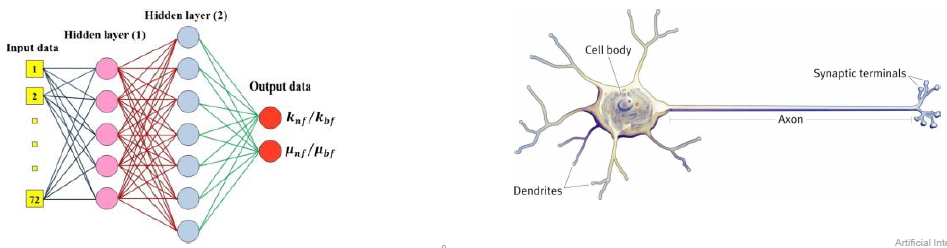
\includegraphics[width=150px]{img/technicalVsBiological.png}
        \captionof{figure}{Abbildung zum Vergleich der Informatik zur Biologie}
        \label{fig:Abbildung zum Vergleich der Informatik zur Biologie}
    \end{Figure}

    \section{Backpropagation}
    Berechne die Gradienten Funktion und propagiere die Änderungen zurück zu den Gewichten, dadurch haben wir eine laufende Anpassung der Gewichtung
    \begin{Figure}
    \centering
    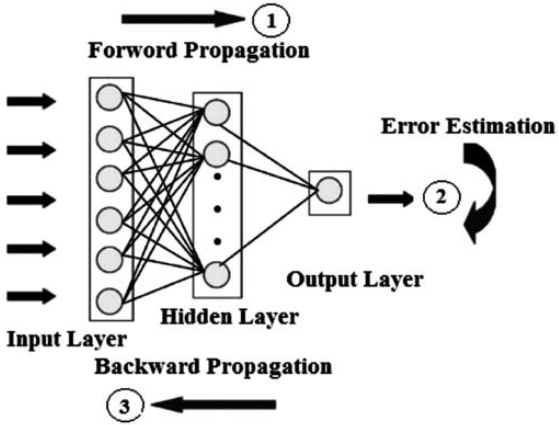
\includegraphics[width=150px]{img/Backpropagation.png}
        \captionof{figure}{Abbildung des Backpropagation-Prozedere}
        \label{fig:Abbildung des Backpropagation-Prozedere}
    \end{Figure}

    Bei einem Multilayer Netzwerk berechnen wir für \textit{for each node: (1) Compute weighted sum of inputs (2) Decide if node is actived}

    \textbf{Nachteile von Backpropagation}
    \begin{itemize}
        \item Erfordert eine große Menge an beschrifteten Trainingsdaten
        \item Bei mehreren verborgenen Schichten ist die Lernzeit langsam
        \item Kann in lokalen Optima stecken bleiben
        \item Problem des verschwindenden Gradienten
    \end{itemize}

    \section{Universality Theorem}
    Das Theorem sagt aus, dass \textit{Ein neuronales Netz mit einer verborgenen Schicht und einer beliebigen Anzahl von Neuronen kann jede beliebige kontinuierliche Funktion approximieren}\\
    \textit{Idee für den Beweis:} Schneiden Sie eine gegebene Funktion g in eine ausreichende Menge kleiner Stücke, dann verwenden Sie 2 Neuronen, die eine partielle lineare Funktion modellieren, um jedes dieser Stücke zu approximieren\\

        \subsection{Schlüsselerfolg: Differenzierbarkeit}
    $\Rightarrow$ Wenn alle Komponenten in einem neuronalen Netz differenzierbar sind, können wir den Gradienten der Leistungsfunktion effizient berechnen
    \begin{Figure}
    \centering
    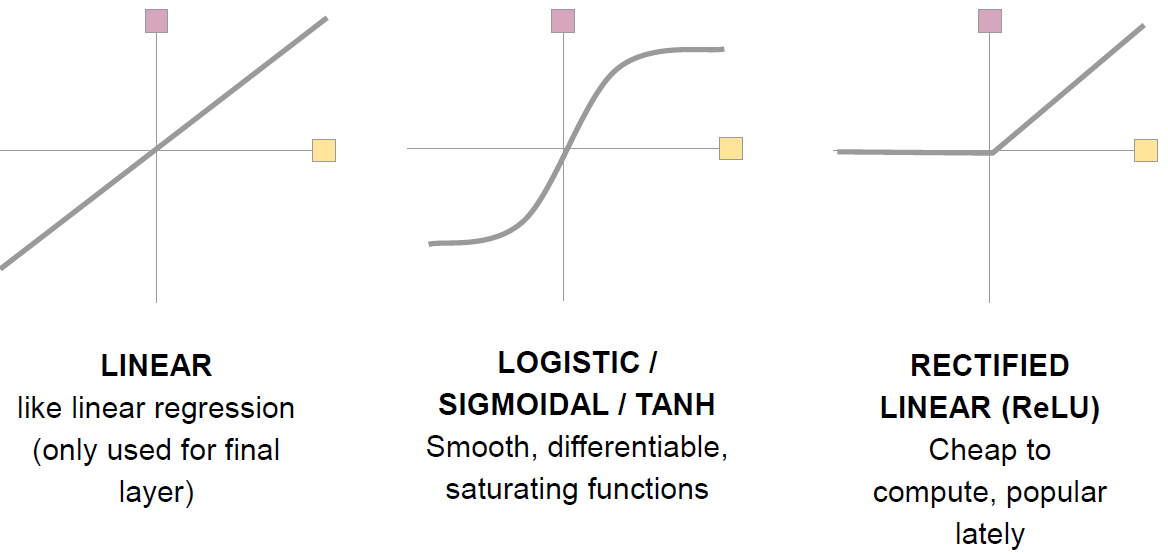
\includegraphics[width=150px]{img/activationFunctions.png}
        \captionof{figure}{Abbildung der verschiednen Aktivierungsfunktionen}
        \label{fig:Abbildung der verschiednen Aktivierungsfunktionen}
    \end{Figure}
    \textbf{Wichtig!} ReLU ist bei 0 nicht differenzierbar, aber wir können einen Wert für die Ableitung 0 oder 1 definieren und dann damit arbeiten.


    \section{Feed-Forward Neural Networks}
    \begin{Figure}
        \centering
        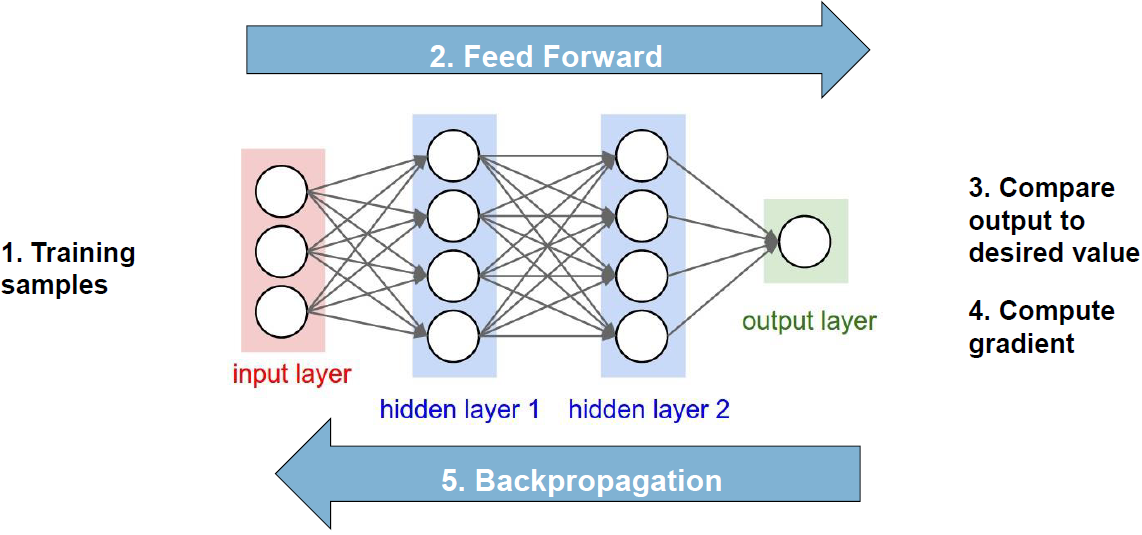
\includegraphics[width=150px]{img/FeedForward.png}
            \captionof{figure}{Abbildung des FeedForward-Prozedere}
            \label{fig:Abbildung des FeedForward-Prozedere}
    \end{Figure}

        \subsection{Vanishing Gradient Problem}

        \subsection{Softmax}
        \textbf{Ziel:} Für den Klassifizierungstask wollen wir eindeutige Klassen, in welchen wir im Outpunkt Layer 1.0 für die korrekte Klasse und 0 für alle anderen Klassen erhalten\\
        \textbf{Idee:} Ein \textit{Max-Layer} setzt 1 für den maximalen Wert vom vorherigen Layer und 0 bei allen anderen Outputs\\
        \textbf{Problem:} Dies ist nicht differenzierbar\\
        \textbf{Lösung:} Eine Softmax-Funktion\\
        \textbf{Bemerkungen:}
        \begin{itemize}
            \item skaliert alle Werte zwischen 0 und 1
            \item Die Summe von allen Werten ist 1, ähnlich wie bei einer Wahrscheinlichkeitsverteilung
            \item Der Maximumswert vom vorherigen Layer wird sehr gross sein im Vergleich zu den anderen Werten
        \end{itemize}
        \begin{Figure}
        \centering
        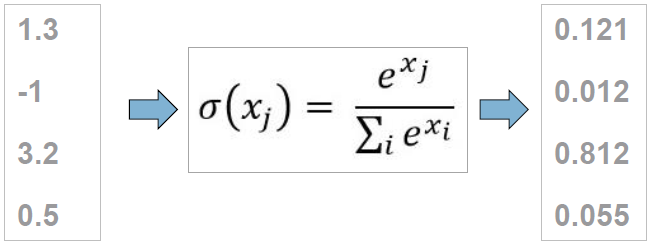
\includegraphics[width=150px]{img/Softmax.png}
            \captionof{figure}{Vor und nach dem Dropout}
            \label{fig:Vor und nach dem Dropout}
        \end{Figure}

        \subsection{Cross-Entropy}
        \textbf{Cross-Entropy Loss}\\
        \textbf{Entropy} Für eine Wahrscheinlichkeitsverteilung $y = (y_1, ..., y_r)$ ist die Entropy $H(y) = \sum^r_{i=1} y_i log(\frac{1}{y_i})$\\
        \textbf{Cross Entropy Loss for one Sample:}\\
        Für ein einziges Samples mit \\ 
        \textit{ground truth Wahrscheinlichkeitsverteilung} $y = (y_1, ..., y_r)$ und \\
        \textit{vorhersagenden Wahrscheinlichkeitsverteilung} $\^y = (\^y_1, ..., \^y_r)$ ist die \\
        \textbf{Cross Entropy Loss} $H(y, \^y) = \sum^r_{i=1} y_i log \frac{1}{\^y_i}$\\
        $\Rightarrow$ Die Cross Entropy ist assymetrisch
        \begin{Figure}
        \centering
        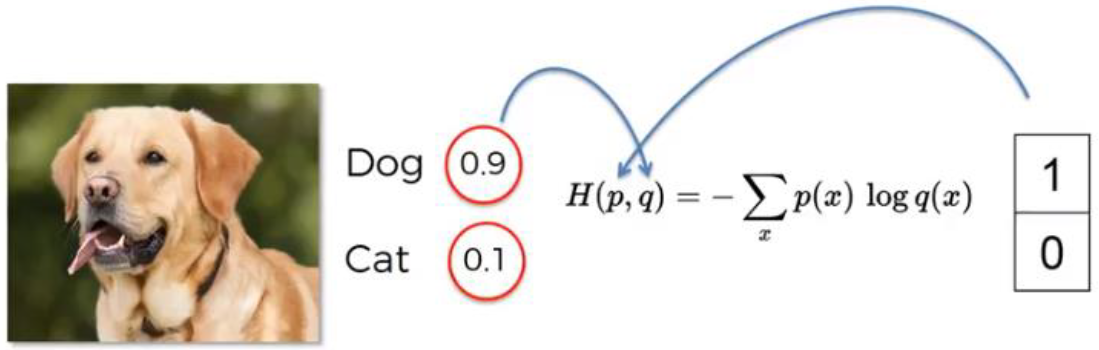
\includegraphics[width=150px]{img/CrossEntropyLoss.png}
            \captionof{figure}{Abbildung Cross Entropy Loss}
            \label{fig:Abbildung Cross Entropy Loss}
        \end{Figure}

        \textbf{Cross-Entropy Cost}
        Für ein set von \textit{n} Sampels, bei dem für jedes gilt\\
        \textit{ground truth Wahrscheinlichkeitsverteilung} $y^{(k)}$ und \\
        \textit{vorhersagenden Wahrscheinlichkeitsverteilung} $\^y^{(k)}$ ist die \\
        \textbf{Cross Entropy Cost Funktion} $H(\{y^{(k)}\}, \{ \^y^{(k)} \}) = \sum^n_{k=1} H(y^{(k)}, \^y^{(k)})$

        $\Rightarrow$ Daumenregel: Verwende Mean-Squarred-Error (MSE) für die Regression und Cross-Entropy für Multiclass-Classification Probleme


        \subsection{Activation Functions}

        \subsection{Dropout}
        \textbf{Ziel:} Vorbeugen von overfitting durch eine bessere Generalisierung\\
        \textbf{Idee:} einen zufälligen Bruchteil von Knoten und entsprechenden Aktivierungen während des Trainings zu ignorieren (Nullung)
        \begin{Figure}
        \centering
        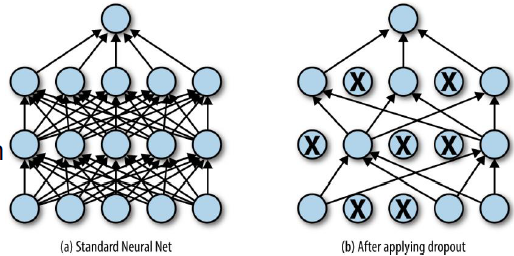
\includegraphics[width=150px]{img/DropoutRegularization.png}
            \captionof{figure}{Vor und nach dem Dropout}
            \label{fig:Vor und nach dem Dropout}
        \end{Figure}

    \section{Keras}


    \section{Convolutional Neural Networks}
    Bei den CNNs vergleicht man nicht Pixel um Pixel, sondern man hat eine Art Fenster, bei welchem auch die benachbarten Pixels miteinbezogen werden. 
    Danach berechnet man die Summe aller Pixel und schreibt diesen in die Feature-Map
    \begin{Figure}
    \centering
    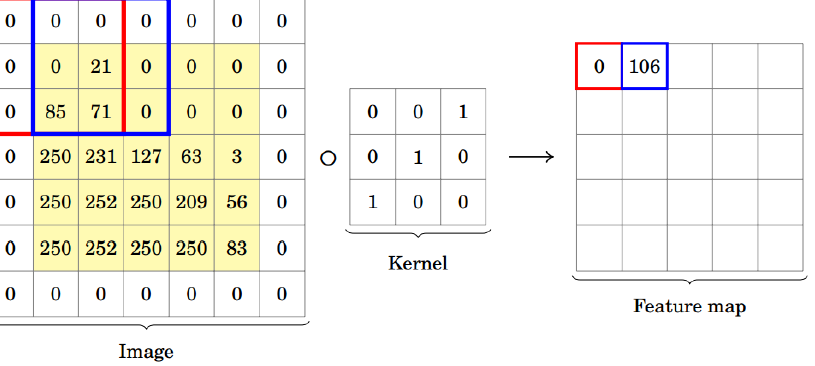
\includegraphics[width=150px]{img/CNN.png}
        \captionof{figure}{Abbildung eines CNNs}
        \label{fig:Abbildung eines CNNs}
    \end{Figure}

    Man trainiert die Werte in einem Filter und verwendet hierzu eine \textit{activationFunctions} für die Erstellung einer Features-Map. Dazu kann man eine oder mehrere Feature-Maps (mit unterschiedlichen Gewichtungen) verwenden.
    Der Standort der Invarianz wird verwendet um bspw. die Edge-Detection abzubilden. 
    \begin{Figure}
    \centering
    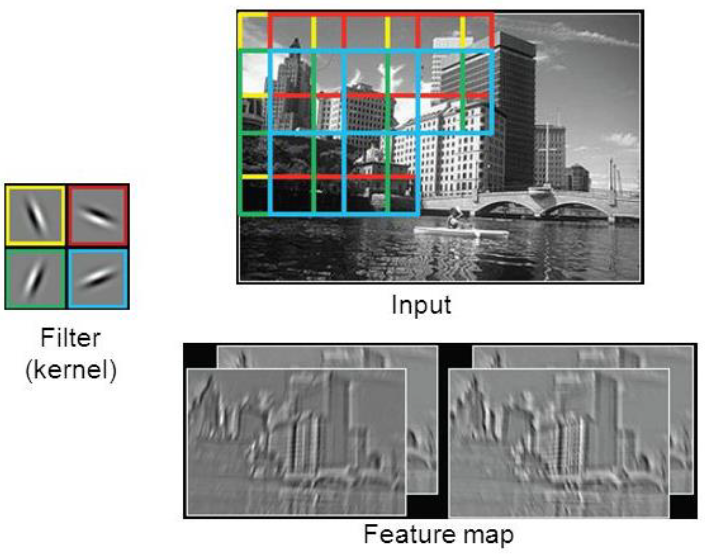
\includegraphics[width=150px]{img/CNNEdgeDetection.png}
        \captionof{figure}{Abbildung eines CNNs mit Edge Detection}
        \label{fig:Abbildung eines CNNs mit Edge Detection}
    \end{Figure}

            \subsubsection{Max Pooling}
    Man reduziert die Bildgrösste durch ein gleitendes Fenster (Sliding Window) ohne Überlappung. Dabei behält man jeweils den maxValue der Pixel. Dies wird auch \textit{sub-sampling} genannt.
    \begin{Figure}
    \centering
    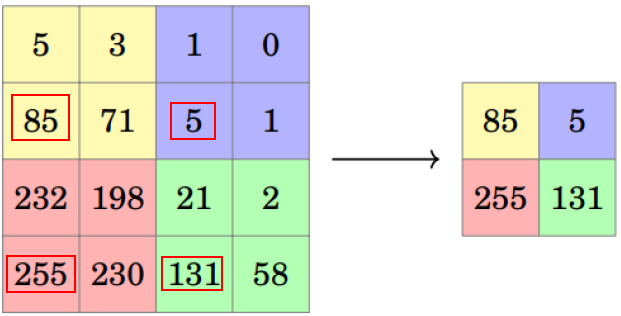
\includegraphics[width=150px]{img/CNNMaxPooling.png}
        \captionof{figure}{Abbildung eines CNNs mittels Max Pooling}
        \label{fig:Abbildung eines CNNs mittels Max Pooling}
    \end{Figure}

        \subsection{CNN für Textanwendungen}
            \subsubsection{Word Embeddings}
            Einfache String als Input funktioniert wirklich gut, daher muss man sich für Text-Analyse etwas mehr gedanken machen. \\
            \begin{itemize}
            \item Multidimensionale Repräsentationen von Wörter
            \item 50-300 Dimensionen sind häufig normal
            \item werden auf Basis eines neuronalen Netzwerkes berechnet
            \item Haben eine dichte Repräsentation (wenig Nullen)
            \item Encoden eine semantische Ähnlichkeit (bspw. Synonyme)
            \item Encoden Analogien (bspw. Distanz zwischen King und Queen ist identisch wie die Distanz zwischen Frau und Mann)
            \end{itemize}

        \subsection{CNN für Textanalyse}
        Gegeben 1 Text und die Word Embeddings\\
        Für jedes Wort haben wir einen Vektor, danach erfolgt ein 1D-Convolution bzw. 2D Convolution $\Rightarrow$ Man erhält einen Vektor und nimmt dabei das Maximum
        $\Rightarrow$ Mehr als 2 Layer bei einem CNN ist nicht sinnvoll bzw. bringt keinen zusätzlichen Wert


    \section{Recurrent Neural Networks (RNNs)}
    RNN's haben eine Art Gedächnis, wo sie speicher, was sie früher bereits einmal berechnet haben. 
    \begin{itemize}
        \item Man verwendet die sequenziellen Informationen
        \item Man führt den Task für jedes Element einer Sequenz durch (\textit{Recurrent} in RNN)
        \item Der Output hängt von den vorherigen Berechnungen ab
    \end{itemize}

        \subsection{Beispiel Text-Character by Character}
        \begin{itemize}
            \item \textbf{Goal} Lerne ein Sprachmodel, welches die Wahrscheinlichkeit von jedem Character vorhersagt, gegeben des vorherigen Characters
            \item Beispiel am Wort \textit{hello}
            \item Um ein Text zu erstellen, starte bei einem zufälligen Character und lass das Netzwerk den nächsten Charakter vorhersagen, dies ist dann der Input für den nächsten Schritt im Netzwerk (RNN)
        \end{itemize}
        
        \begin{Figure}
        \centering
        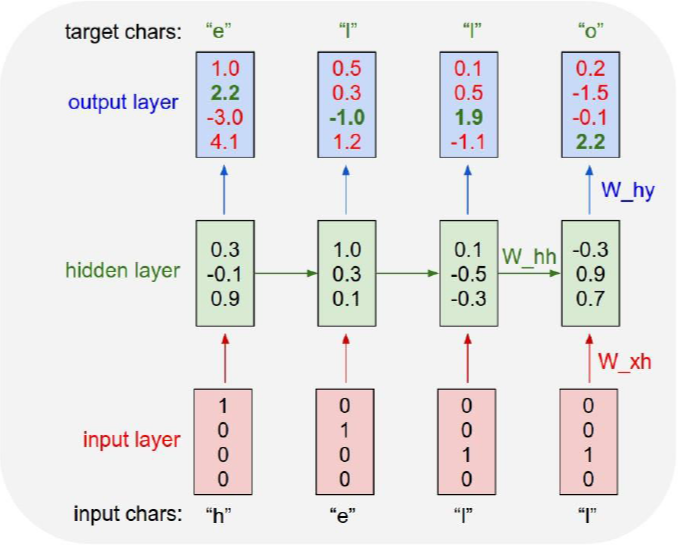
\includegraphics[width=150px]{img/RNNHello.png}
            \captionof{figure}{Beispiel eines RNN mit dem Wort Hello}
            \label{fig:Beispiel eines RNN mit dem Wort Hello}
        \end{Figure}
    
        \subsection{Beispiel Sentiment Analyse}
        \begin{Figure}
        \centering
        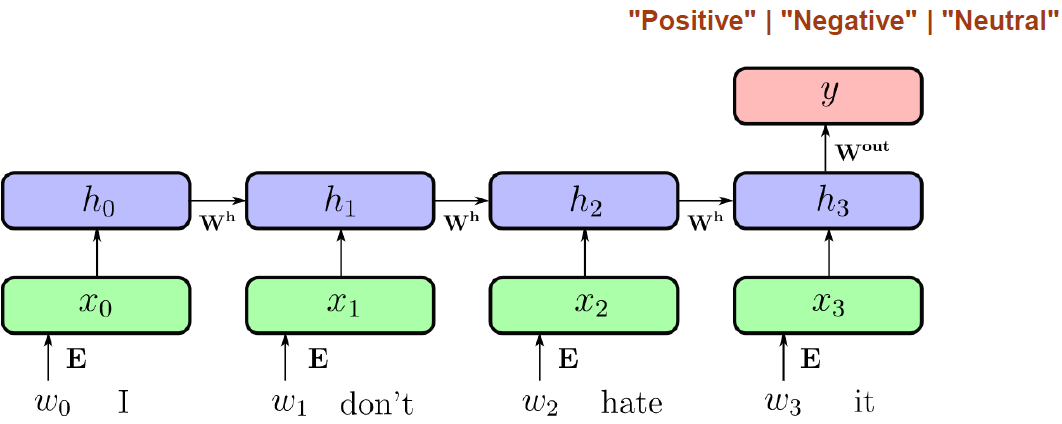
\includegraphics[width=150px]{img/RNNSentiment.png}
            \captionof{figure}{Beispiel eines RNN für die Sentiment Analyse}
            \label{fig:Beispiel eines RNN für die Sentiment Analyse}
        \end{Figure}
        
        \begin{Figure}
        \centering
        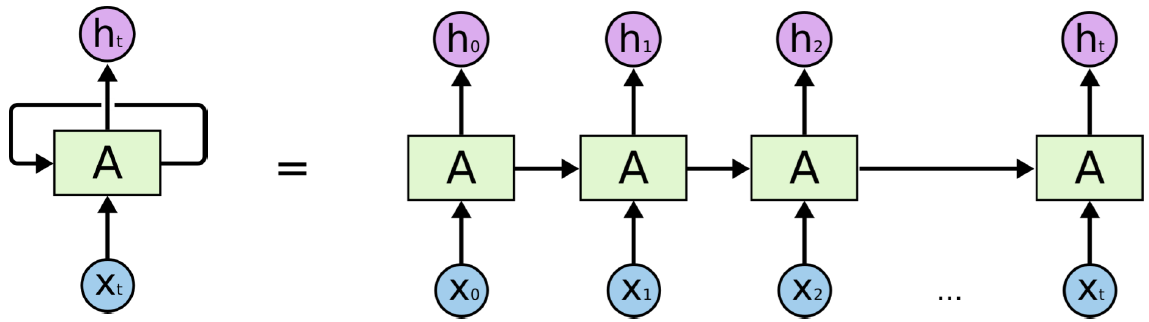
\includegraphics[width=150px]{img/RNNStructure.png}
            \captionof{figure}{Abbildung der Struktur eines RNNs}
            \label{fig:Abbildung der Struktur eines RNNs}
        \end{Figure}
        $\rightarrow$ \textbf{$x_t$} ist der Input zum Zeitpunkt \textit{t}, \textbf{$h_t$} ist der Output zu diesem Zeitpunkt\\
        $\rightarrow$ ist das Model, welches repetiert wird. In jedem A wird das gleiche Neural Network verwendet.
        
        \subsection{Langzeit Abhängigkeit}
        Dies beschreibt die Abhängigkeit in einem langen Satz. Wenn wir innerhalb eines Satzes, das nächste Wort vorhersagen möchten.\\
        Ein Problem dabei ist, dass das Gedächtnis sehr "kurzfristig" ist. Jeder Wert, der in einem Zeitschritt ausgegeben wird, wird im nächsten Schritt eingegeben, aber wenn derselbe Wert nicht wieder ausgegeben wird, geht er beim nächsten Schritt verloren.\\
        $\Rightarrow$ Theoretisch wäre dies möglich, in der Praxis ist dies aber nicht möglich!
        
        \begin{Figure}
        \centering
        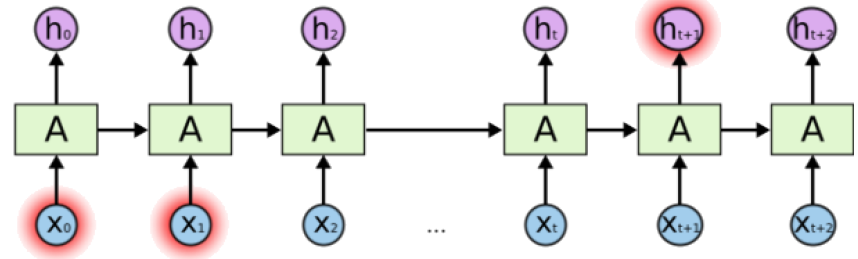
\includegraphics[width=150px]{img/RNNLongTerm.png}
            \captionof{figure}{Abbildung der Struktur eines longterm RNNs}
            \label{fig:Abbildung der Struktur eines longterm RNNs}
        \end{Figure}
    \section{RNNs with Long Short Term Memory Networks (LSTM)}
    \begin{itemize}
        \item Spezielle Form von RNNS
        \item Explizit für das Problem der langzeit-Abhängigkeit entwickelt
        \item erinnert sich an Informationen für eine lange Zeit
        \item Löst das Vanishing Gradient Problem von RNNs
        \item RNNs mit einem Speicher und einem \textit{Gating Mechanismum} für Input, forget, output
        \item funktioniert für viele Anwendungsfälle und ist in weitem Gebraucht
        \item Können tausende von Zeitschritten unterhalten
        \item gibt verschiedene Variante (Peephole Connections, Gated Recurrent Units (GRU), Bi-directional LSTMs etc.)
    \end{itemize}
    \begin{Figure}
    \centering
    \includegraphics[width=150px]{img/LSTM.png}
        \captionof{figure}{Abbildung der Struktur eines LSTM}
        \label{fig:Abbildung der Struktur eines LSTM}
    \end{Figure}
        
        \subsection{Aufbau von LSTM}
        
            \subsubsection{Notation}
            \begin{Figure}
            \centering
            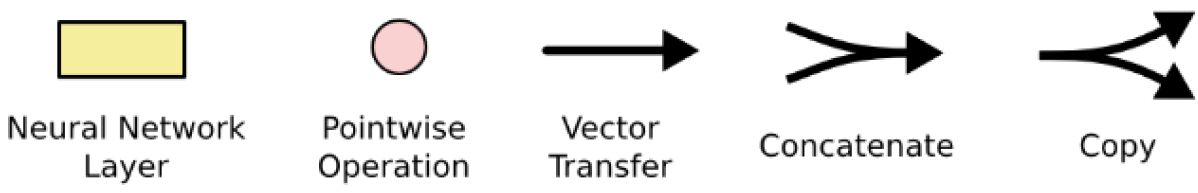
\includegraphics[width=150px]{img/LSTMNotation.png}
                \captionof{figure}{Notation eines LSTM}
                \label{fig:Notation eines LSTM}
            \end{Figure}
        
            \subsubsection{Kernidee}
            \begin{itemize}
                \item Schlüssel für den Erfolg ist der Cell State \textbf{$C_t$}, welches einen Vektor darstellt
                \item LSTM kann Informationen diesem Cell State hinzufügen oder löschen
                \item Dies geschieht über die regulierte Struktur der Gates
                \item LSTM haben drei Gates für den Schutz und Kontrolle des Cell State
            \end{itemize}
            \begin{Figure}
            \centering
            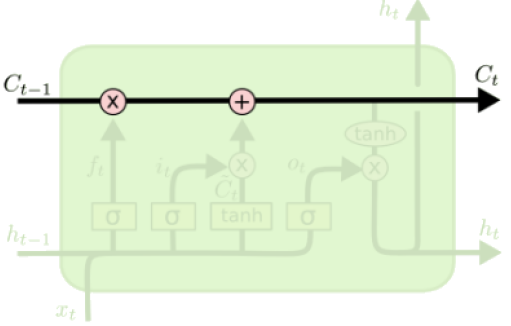
\includegraphics[width=150px]{img/LSTMCellState.png}
                \captionof{figure}{Abbildung des Cell State in LSTM}
                \label{fig:Abbildung des Cell State in LSTM}
            \end{Figure}
        
            \subsubsection{Forget Gate}
            \begin{itemize}
                \item Das Forget-Gate entscheidet welche Information verworfen werden
                \item Schaut bei $h_{t-1}$ und $x_t$ und generiert einen Output zwischen 0 und 1
                \item 1 repräsentiert, dass die Information behaltet werden soll
                \item 0 repräsentiert, dass die Information verowrfen werden kann
                \item Falls $f_t$ 0 ist an einem Eingang, dann wird der Eingang von $C_{t-1}$ vollständig gelöscht
            \end{itemize}
            \begin{Figure}
            \centering
            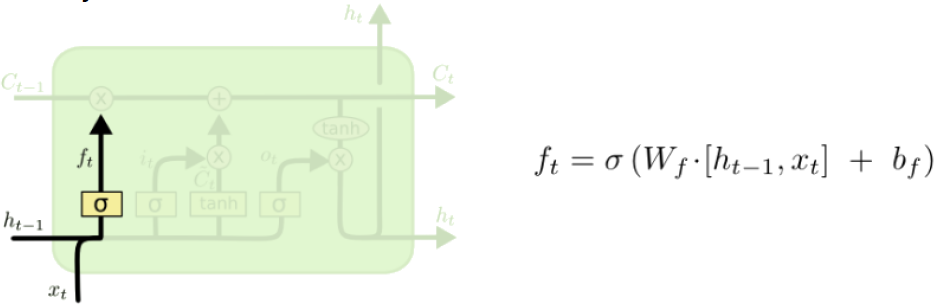
\includegraphics[width=150px]{img/LSTMForgetGate.png}
                \captionof{figure}{Abbildung des Forget Gates in LSTM}
                \label{fig:Abbildung des Forget Gates in LSTM}
            \end{Figure}
        
            \subsubsection{Input Gate}
            \begin{itemize}
                \item das Input-Gate entscheidet, welche neue Informationen im Cell State gespeichert werden sollen
                \item 1. Part: Ein sigmoid-Layer (Input gate layer): Entscheidet welcher Wert $i_t$ wir updaten sollen
                \item 2. Part: ein tanh-Layer: Erstellt einen Vektor, welcher ein neuer candidate value ist $\rightarrow$ $\~C_t$
            \end{itemize}
            \begin{Figure}
            \centering
            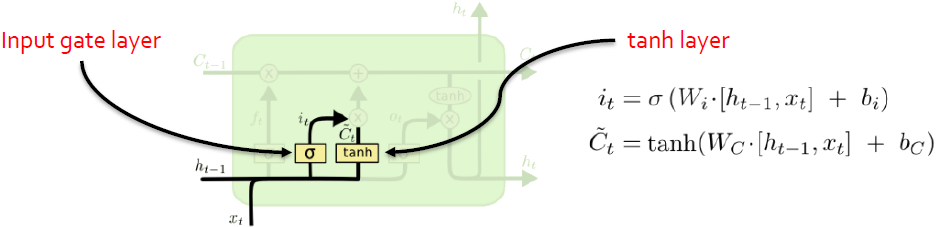
\includegraphics[width=150px]{img/LSTMInputGate.png}
                \captionof{figure}{Abbildung des Input Gates in LSTM}
                \label{fig:Abbildung des Input Gates in LSTM}
            \end{Figure}
        
            \subsubsection{Update Cell State}
            \begin{itemize}
                \item updatet der Alte-Status von $C-{t-1}$ in den neuen Cell state $C_t$
                \item 1. Operation - Multiply: Multipliziert den alten Status von $f_t$ (Vergisst die Dinge, welche mir früher entschieden haben zu vergessen)
                \item 2. Operation - Add: addiert $i_t * \~C_t$
            \end{itemize}
            \begin{Figure}
            \centering
            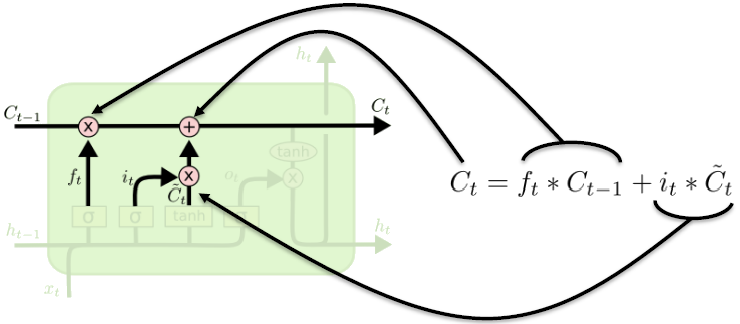
\includegraphics[width=150px]{img/LSTMUpdateGate.png}
                \captionof{figure}{Abbildung des Update Gates in LSTM}
                \label{fig:Abbildung des Update Gates in LSTM}
            \end{Figure}
        
            \subsubsection{Output Generation}
            \begin{itemize}
                \item Das Output-Gate entscheidet was wir als Output liefern
                \item 1. Step: Wir lassen den Sigmoid-Layer laufen, welcher entscheidet welche Abschnitt des Cell-States als Output ($o_t$) geliefert werden sollen
                \item 2. Step: Wir lassen den Cell-State durch den tanh-Layer laufen und multiplizieren diesen mit dem Output des sigmoid-Layer
                \item 3. Step: Output and Cell-State are passed on as new input for the next step 
            \end{itemize}
            \begin{Figure}
            \centering
            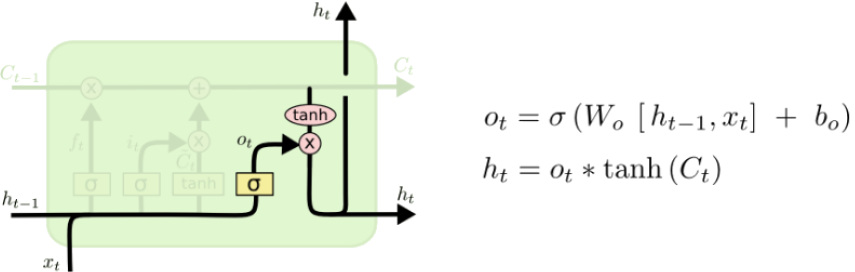
\includegraphics[width=150px]{img/LSTMOutputGeneration.png}
                \captionof{figure}{Abbildung der Output Generatino in LSTM}
                \label{fig:Abbildung der Output Generatino in LSTM}
            \end{Figure}
        \subsection{RNN vs. LSTM}
        \begin{Figure}
        \centering
        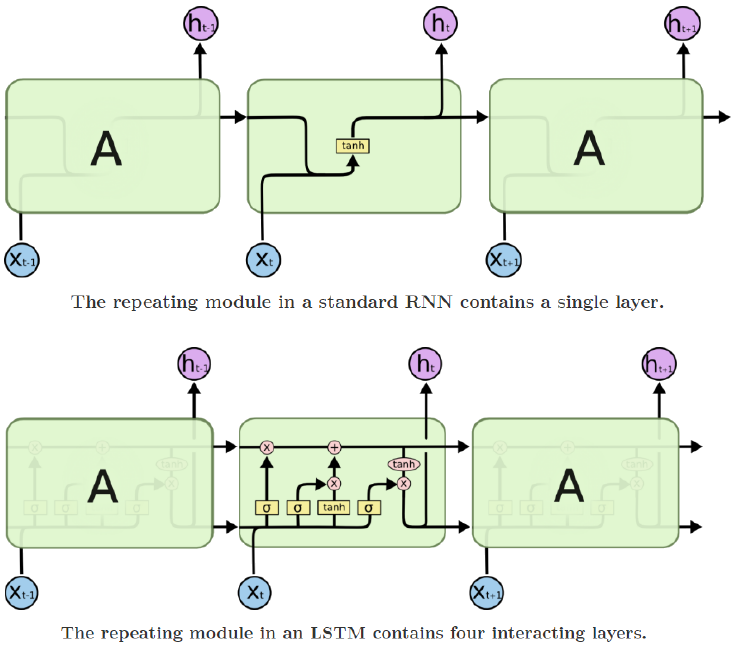
\includegraphics[width=150px]{img/RNNvsLSTM.png}
            \captionof{figure}{Strukturvergleich zwischen RNN und LSTM}
            \label{fig:Abbildung der Struktur eines LSTM}
        \end{Figure}


    \section{Neural Network Architecture Quiz}
%ToDo Antworten einfügen

    \section{Dialogue Systems}
    \textbf{Definition Conversational Diaologue Systems (Chatbots) :=} Allow users to chat in a natural way about arbitrary topics

	    \subsection{Recap Generative Adversial Netwroks (GANs)}
        \begin{Figure}
        \centering
        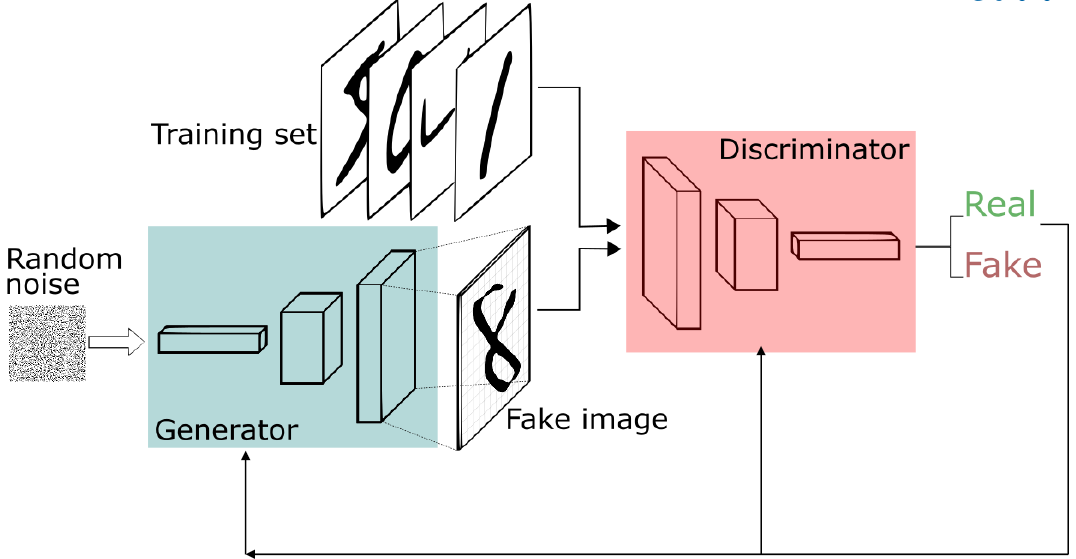
\includegraphics[width=150px]{img/GAN.png}
            \captionof{figure}{Abbildung eines GANs}
            \label{fig:Abbildung eines GANs}
        \end{Figure}

	    \subsection{Stereotypes of Dialogue Systems}
        \begin{itemize}
            \item Question-Answering (bspw. Who was the director of Titanic?)
            \item Pro-Active Dialogue Systems (bspw. Hast du Fieber?, ..., Diagnose)
            \item Conversational Agents (Chatbot) (bspw. Was ist dein Name, etc.)
        \end{itemize}

	    \subsection{Chatbots}
        Hauptgründe wieso Chatbots fehlschlagen
        \begin{itemize}
            \item Vereinfacht nicht den Task
            \item Keine Interaktion mit anderen Systemen
            \item Schwacher Use-Case
            \item Zu ambitioniert
        \end{itemize}

	    \subsection{Komponenten eines Dialog Systems}
        \textbf{Speech to Text}
        \begin{itemize}
            \item Intent Classification
            \item Enitity Recognition
            \item Context Tracking
        \end{itemize}

        \textbf{Text to Speech}
        \begin{itemize}
            \item Answer Selection
            \item Slot-Filling
            \item Natural Language Generation
        \end{itemize}

        Betrachtet man die Entwicklung eines Conversational Systems, dann kann man folgende Daumenregel anwenden:
        \begin{itemize}
            \item Training Data $\rightarrow$ Millionen von real-world Dialoge
            \item Technologie $\rightarrow$ Deep Neural Network ('Sequence2Sequence')
            \item Training Time $\rightarrow$ einige Wochen
        \end{itemize}
        \begin{Figure}
        \centering
        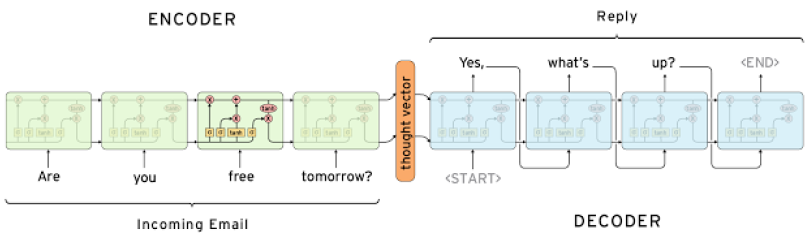
\includegraphics[width=150px]{img/MakingConvSystem.png}
            \captionof{figure}{Abbildung des Vorgehens eines Conversational Systems}
            \label{fig:Abbildung des Vorgehens eines Conversational Systems}
        \end{Figure}


\chapter{Reinforcement Learning}
$\rightarrow$ Ganz andere Denkweise zu Deep Learning\\
$\Rightarrow$ Wählt diesen Status aus, welchen den Reward in der GESAMTHEIT zu maximieren 


Aus Erfahrungen mit der Interaktion der Umwelt, lernt wie man Probleme lösen kann $\rightarrow$ Das Ziel ist mit möglichst wenig Daten bereits ein sehr mächtiges Model erstellen können\\
Analogie zum Velo fahren lernen: Man kann es nicht durch Youtube-Videos oder Erklärungen erlernen. Sondern es ist ein Trial-Error-Verfahren. Dabei sind die viele verschiedenen Faktoren relevant.
\begin{Figure}
\centering
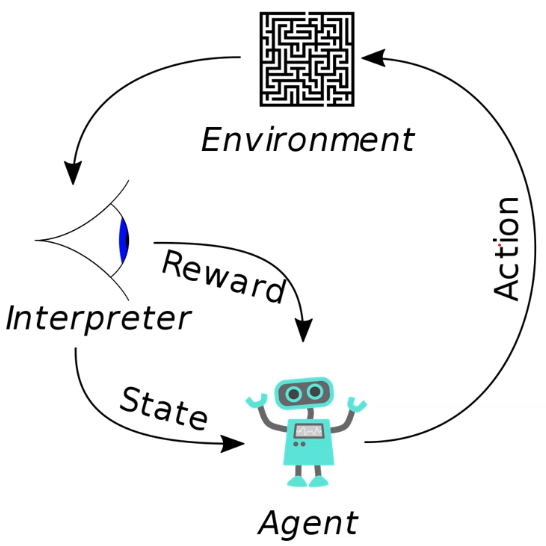
\includegraphics[width=150px]{img/ReinforcementLearningModel.png}
	\captionof{figure}{Abbildung zum Ablauf von Reinforcement Learning}
	\label{fig:Abbildung zum Ablauf ovn Reinforcement Learning}
\end{Figure}

Das Model erhält durch die Handlungen positive bzw. negative Rewards. Wenn es ein sehr negativer Reward ist, dann stribt der Spieler. Dadurch lernt das System von mal zu mal immer besser wie das Spiel funktioniert.\\
Bei den Atari Spielen war der Durchbruch, dass der Computer keine informationen zu den Spielen erhalten hat, sondern sich alles selbstständig beigebracht hat - durch Beobachtung der Umwelt.

\section{Schritte für das Erstellen von Reinforcement Systeme}
\begin{enumerate}
	\item Formuliere das Problem: goal, environment, states, actions, rewards 
	\item Bestimme das environment: real-world oder simuliert
	\item Wähle oder implementiere den Trainings-Algorithmus und die value-function $\rightarrow$ Erhält nur die notwendigsten Informationen Bspw. Goal und environment, aber sicherlich nicht die rewards
	\item Episodenweise Durchführung $\rightarrow$ Erkunden des environment um das Modell zu trainieren
\end{enumerate}

	\subsection{Goal}
Gegeben dem \textbf{aktuellen Status}, eine \textbf{Aktion zu wählen} um in Zukunft alle \textbf{totalen Rewards zu maximieren} \\
$\rightarrow$ Manchmal macht es Sinn einen Umweg zu gehen und auf gewisse Rewards zu verzichte, um in Zukunft die Rewards zu maximieren

\section{Reinforcement Agent}
Was steuert das Verhalten meines Agenten?
\begin{enumerate}
	\item policy $\pi$ $\rightarrow$ Algorithmus $\Rightarrow$ Ist das grundsätzliche Ziel, jedoch hilft hierzu das Model bzw. value-Function
	\item value-Funktion $v$ oder $q$ $\rightarrow$ Wie gut ist der aktuelle state bzw. Action $\Rightarrow$ Mit einer guten value-Funktion gibt es eine gute policy
	\item Model $\rightarrow$ Agenten-Repräsentation des Environments $\Rightarrow$ Gibt den Wert von bspw. jedem Feld und gibt eine gute Wert-Funktion
\end{enumerate}

    \section{Markov Decision Processes}
    \begin{Figure}
    \centering
    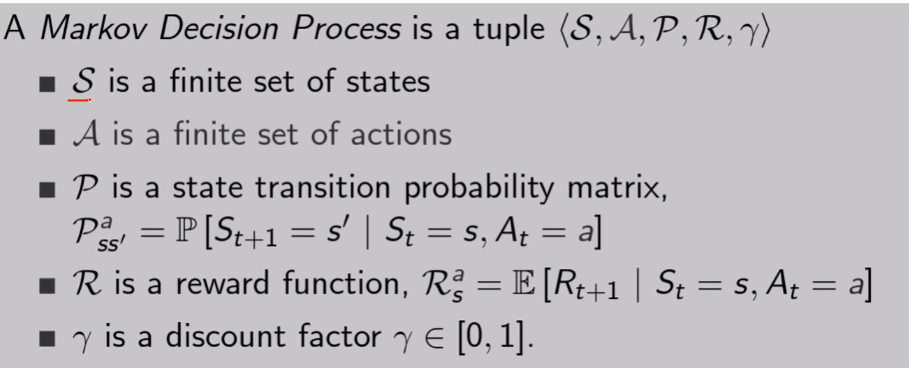
\includegraphics[width=150px]{img/MDP.png}
        \captionof{figure}{Abbildung zur Beschreibung zu Markov Decision Process}
        \label{fig:Abbildung zur Beschreibung zu Markov Decision Process}
    \end{Figure}
        
    \begin{Figure}
    \centering
    \includegraphics[width=150px]{img/MDPStudentBehvaiour.png}
        \captionof{figure}{Abbildung zu einem beispielhaften MDP mit dem Verhalten von Studierenden}
        \label{fig:Abbildung zu einem beispielhaften MDP mit dem Verhalten von Studierenden}
    \end{Figure}

        \subsection{policy}
        die Policy $\pi$ ist eine Verteilung über die Aktionen von gegebenen States.\\
        \begin{itemize}
            \item Eine Policy definiert das Verhalten eines Agent vollständig
            \item MDP-Policies hängen vom aktuellen State ab (nicht von der History)
        \end{itemize}
        
        \begin{equation}
        \pi (a | s) = \mathbb{P} [A_t = a | S_t = s]
        \end{equation}

            \subsubsection{Transition Proabilitied and Rewards under a policy}
            Gegeben einer Policy $\pi$, können wir die Übergangswahrscheinlichkeit und den Reward berechnen
            
            \begin{equation}
            \begin{split}
                P^\pi_{s, s'} &= \sum_{a \in A} \pi(a|s) P^a_{ss'}
                R^\pi_s &= \sum_{a \in A} \pi (a|s) R^a_s
            \end{split}
            \end{equation}
            
                \subsection{Return}
            \textit{return} $G_t$ ist der discounted Reward für den Zeitschritt $t$
            \begin{equation}
                G_t = R_{t+1} + \gamma R_{t+2} + ... = \sum_{k=0}^{\inf} \gamma^k R_{t+k+1}
            \end{equation}
            
            \begin{itemize}
                \item Der Discount $\gamma \in \[0,1\]$ ist der present-value of future rewards
                \item der Wert der Belohnung nach k+1 Zeitschritten beträgt $\gamma^k R$
                \item Dieser Wert der sofortige Belohnung ist höher als die verzögerte Belohnung $\rightarrow$ $\gamma$ nahe bei 0 führt zu 'myopic' evaluation $\rightarrow$ $\gamma$ nahe bei 1 führt zu 'far-sighted' evaluation
            \end{itemize}
            
            $\rightarrow$ Finde eine policy $\pi*$ welche den \textbf{return $G_0$} maximiert.
            
            \subsubsection{Rekurisver Ausdruck von $G_t$}
            Der Return zum Zeitpunkt $t$ ist
            \begin{equation}
                \begin{split}
                    G_t &= R_{t+1} + \gamma R_{t+2} + \gamma^2 R_{t+3} + \gamma^3 R_{t+4} + \dots \\
                    &= R_{t+1} + \gamma(R_{t+2} + \gamma^1 R_{t+3} + \gamma^2 R_{t+4} + \dots) \\
                    &= R_{t+1} + \gamma G_{t+1}
                \end{split}
            \end{equation}

                \subsection{Discount Factor $\gamma$}
            \begin{itemize}
                \item $0 \leq \gamma \leq 1$
                \item discounts future rewards
                \item typischer Wert ist $\gamma = 0.9$ oder $\gamma = 0.99$
            \end{itemize}

                \subsection{Discounted Rewards}
            Wieso werden viele Markov-Entscheidungen diskontiert?
            \begin{itemize}
                \item Mensch und Tier haben eine Präferenz für sofortige Belohnungen
                \item Wenn es sich um eine finanzielle Belohnung handelt, können sofortige Belohnungen mehr Zinsen einbringen als verspätete Belohnungen
                \item Es ist mathematisch gesehen, angenehmen Rabatte (Discounts) zu gewähren
                \item Vermeide unendlich returns in zyklischen Markov Prozessen
            \end{itemize}

    \section{Value Functions}
        \subsection{action-Value Functions}
        \textbf{Definition:} Die \textit{action-value Function} $q_{\pi} (s,a)$ ist der erwartende Return, beginnendend beim State $s$, mit der Aktion $a$ und der Policy $\pi$
        \begin{equation}
            q_\pi(s,a) = \mathbb{E}_\pi [G_t | S_t = s, A_t = a]
        \end{equation}
        \textit{Hinweis:} In der action-value function wird die Aktion $a$ nicht durch die Richtlinie $\pi$ gewählt, sondern kann eine beliebige Aktion sein

        \subsection{State-Value Function}
        \begin{equation}
            v_\pi (s) = E_\pi [G_t | S_t = s]
        \end{equation}

    \section{Policy Iteration}
    Define a partial ordering over policies: $\pi \geq \pi' if v_\pi (s) \geq v_{\pi'}(s), \forall s $\\
    \textbf{Theorem:}\\
    Für jeden Markov Decision Process:
    \begin{itemize}
        \item existiert eine optimale Policy $\pi_*$, welche besser oder gleich zu allen anderen Policies ist, $\pi_* \geq \pi, \forall \pi$
        \item Alle optimalen Policies erreichen die optimale action-value Function $q_{\pi_*}(s,a) = q_*(s,a)$
    \end{itemize}
    
        \subsection{Finden der optimalen Policy}
    Die optimale Policy kann gefunden werden, in dem man eine Maximierung von $q_* (s,a)$ findet
    \begin{numcases}{$\pi_* (a|s)$}
        1, & wenn $a = argmax_{a \in A} q_* (s,a)$\\
        0, & sonst 
    \end{numcases}
    Es gibt immer eine deterministische optimale Policy für jeden MDP (Markov Decision Process)\\
    $\Rightarrow$ Wenn wir $q_*(s,a)$ kennen, haben wir sofort auch die optimale Policy!


    \section{$\epsilon$-Greedy Exploration}

    \begin{itemize}
        \item Ist die einfachste Idee die kontinuierliche Exploration zu gewährleisten
        \item alle $m$ Aktionen werden mit einer non-zero Wahrscheinlichkeit versucht
        \item Mit der Wahrscheinlichkeit $1-\epsilon$ wird die greedy-Action ausgewählt
        \item Mit der Wahrscheinlichkeit $\epsilon$ wird eine Aktion nach dem Zufallsprinzip ausgewählt
    \end{itemize}
    
    \begin{numcases}{$\pi (a*|s)$}
        $\frac{\epsilon}{m+1-\epsilon}$, & wenn $a* = argmax_{a \in A} Q (s,a)$\\
        $\frac{\epsilon }{m}$, & sonst 
    \end{numcases}
    $\Rightarrow$ In Schritt k einer Episode können wir $\epsilon = \frac{1}{k}$ verwenden, um mit der Zeit von der Exploration zur Ausbeutung überzugehen
    

        \subsection{Exploration vs. Exploitation}
        Exploration $\Rightarrow$ Taking a change to learn new things\\
        Exploitation $\Rightarrow$ What you have learned

        \begin{itemize}
            \item Die nächste action auszuwählen ist ein balancierter Akt zwischen \textit{exploration} und \textit{exploitation}
            \item Wenn man immer exploration auswählt, rennt man allenfalls sehr häufig in Probleme rein
            \item Wenn man immer exploitation auswählt, erreicht man allenfalls nie 'high-value rewards'
            \item Zu Beginn, kann der Agent etwas mehr untersuchen (explore) für eine zufällige Anzahl episoden ($\Rightarrow$ heatup phase) und danach fokussierte greedy-Entscheide treffen 
        \end{itemize}

    \section{Model-Based Learning}
    Beim \textbf{Model-based Learning} kennen wir die Zustandsübergangswahrscheinlichkeiten \textbf{P} und die Belohnungsfunktion (Reward Function) \textbf{R} eines MDP.\\
    In diesem Fall können wir eine gegebene Policy $\pi$ durch eine \textit{Policy Iteration} verbessern:
    \begin{enumerate}
        \item gegeben P,R, $\pi \rightarrow$ berechne v,q
        \item gegeben $\pi$ und v,q $\rightarrow$ erstelle eine bessere Policy $\pi'$
    \end{enumerate}

        \subsection{Bellman Equations for Value Functions}
    \begin{equation}
        \begin{split}
            v_\pi(s) &= \sum_{a \in A} \pi(a|s) (R^a_s) + \gamma \sum_{s' \in S} P^a_{ss'}v_\pi(s') \\
            q_\pi(s,a) &= R^a_s + \gamma \sum_{s'\in S} P^a_{ss'} \sum_{a' \in A} \pi(a'|s') q_\pi(s', a')
        \end{split}
    \end{equation}

        \subsection{Greedy Policy Improvement}
        Gegeben einer Policy $\pi$ und seiner state-value function $v_\pi$, können wir eine neue (nicht zwingend optimale) Policy $\pi'$  mit dem \textit{greedy policy improvement} kreiieren:
        \begin{equation}
            \pi' (s) = argmax_{a \in A} R^a_s + P^a_{ss'} V(s')
        \end{equation}
        $\Rightarrow$ Die neue Policy $\pi'$ ist mindestens so gut wie $\pi$
        
        \begin{itemize}
            \item \textbf{Policy evaluation} estimate $v_\pi$ iterative policy evaluation
            \item \textbf{Policy Improvement} Generate $\pi' \geq \pi$ Greedy policy improvement
        \end{itemize}
        \textbf{Wichtig!} Der Prozess des \textit{greedy policy iteration} mit bekanntem \textbf{R} und \textbf{P} konvergiert \textbf{immer} zu einer optimalen policy $\pi^*$
        
        \begin{Figure}
            \centering
            \includegraphics[width=150px]{img/greedyPolicyIteration.png}
                \captionof{figure}{Abbildung der Policy Iteration}
                \label{fig:Abbildung der Policy Iteration}
        \end{Figure}

    \section{Model-Free Predication}
    Beim \textbf{Model-free Learning}, kennen wir die MDP-Paramter \textbf{nicht} (wie bspw. die Übergangswahrscheinlichkeit P und die reward-Function R).\\
    $\rightarrow$ in diesem Fall, können wir die value-function $v$, sowie das $q$ einer Policy $\pi$ nur schätzen,in dem man eine oder mehrere Epsioden des MDP mit $\pi$ durchläuft.

        \subsection{Monte-Carlo (MC)}
        \begin{itemize}
            \item MC Methoden lernen direkt aus den Erfahrungen der Episoden
            \item MC ist ein model-free Learning $\rightarrow$ Es gibt keine Kenntnisse von MDP-Übergang/Belohnungen
            \item MC lernt aus \textit{kompletten} Episoden
            \item MC verwendet die einfachstmöglichste Idee
            \item \textbf{Vorbehalt:} Monte-Carlo Learning kann nur auf episodische MDPs angewendet werden und alle Episoden müssen beendet werden
        \end{itemize}

        \subsection{Temporal Difference Learning (TD)}
        \begin{itemize}
            \item TD Methoden lernen direkt aus den Erfahrungen der Epsioden
            \item TD ist ein model-free LEarning $\rightarrow$ Es gibt keine Kenntnisse von MDP-Übergang/Belohnung
            \item TD lernt aus \textit{unvollständigen} Episoden $\rightarrow$ durch Bootstrapping
            \item TD aktualisiert eine Vermutung in Richtung einer Vermutung
            \item Einfachster Zeitdifferenz-Lernalgorithmus: TD(0)
            \item Wert $V(S_t)$ wird zum geschätzen Return \textbf{$R_{t+1} + \gamma V(S_{t+1})$} aktualisiert: $V(S_t) \leftarrow V(S_t) + \alpha (\textbf{R_{t+1} + \gamma V(S_{t+1})} - V(S_t))$
        \end{itemize}
       
        \begin{Figure}
           \centering
           \includegraphics[width=150px]{img/TDLearning.png}
               \captionof{figure}{Abbildung des TD Learning}
               \label{fig:Abbildung des TD Learning}
       \end{Figure}
       
       \textbf{Hinweis:} Q-Learning ist ein TD-Learning, da man einen Schritt vorausschaut und nimmt den aktuellen Zustand für das Update zu machen.
       
    
    \section{Q-Learning}
    Q-Learning verfolgt das Ziel die Policy zu maximieren
    \begin{Figure}
    \centering
    \includegraphics[width=150px]{img/QLearning.png}
        \captionof{figure}{Abbildung zum Q-Learning Algorithmus}
        \label{fig:Abbildung zum Q-Learning Algorithmus}
    \end{Figure}

    \begin{itemize}
        \item Q-Funktion $Q(s,a)$ mit Zustand (State) und Aktion $\rightarrow$ Sagt uns wie gut jede Aktion im aktuellen Zustand ist (bspw. Greedy)
        \item terminal-States da wird das Spiel beendet
        \item epidose: Spiel einmal durchlaufen lassen
    \end{itemize}

    \begin{Figure}
    \centering
    \includegraphics[width=150px]{img/QFunktion.png}
        \captionof{figure}{Ablauf zum Q-Learning}
        \label{fig:Ablauf zum Q-Learning}
    \end{Figure}
    
    $\Rightarrow$ Bei genügend Durchläufe konvergiert Q zu einer optimalen Q-Funktion $\rightarrow$ mit maximiertem Reward
    
        \subsection{Learning Q}
    \begin{itemize}
        \item Ziel von Q-Learning ist zu Q zu lernen mit der 'Action-value Function'
        \item Q ratet wie viel Reward erwartet werden kann, wenn eine bestimmte Aktion durchgeführt wird
        \item Gegeben eines guten Q, ist es sehr einfach eine gute policy für den Agenten zu konstruieren
        \item Q-Learning konvergiert zu einem optimalen Q
    \end{itemize}     

    \section{SARSA}

    \begin{equation}
        Q(S,A) \leftarrow Q(S,A) + \alpha (R+\gamma Q(S',A') - Q(S,A))
    \end{equation}
    
    \textbf{Theorem:} SARSA konvergiert zur optimalen Aktionswertfunktion $Q(s,a) \rightarrow q^*(s,a)$, unter bestimmten vernünftigen Bedingungen
    
    \begin{Figure}
        \centering
        \includegraphics[width=150px]{img/SARSA.png}
            \captionof{figure}{Abbildung des SARSA-Schemas}
            \label{fig:Abbildung des SARSA-Schemas}
    \end{Figure}
    
    \begin{Figure}
        \centering
        \includegraphics[width=150px]{img/SARSAPseudoCode.png}
            \captionof{figure}{Abbildung des SARSA PseudoCodes}
            \label{fig:Abbildung des SARSA PseudoCodes}
    \end{Figure}
    
        \subsection{SARSA vs. Q-Learning}
        SARSA folgt einfach der aktuellen Policy, die nächste Aktion aus $S'$ auszuwählen, während bei Q-Learning das Maximum von $Q$ über alle möglichen Aktionen aus Zustand $S'$ verwendet wird.
 \end{document}